\documentclass[10pt,a4paper]{article}
\newcommand{\runningtitle}{Conditional flow matching in acute human wounds}
\usepackage[margin=15mm,top=16mm,bottom=17mm,headheight=12pt,headsep=5mm,footskip=9mm]{geometry}
\usepackage{fontspec}
\setmainfont{TeX Gyre Termes}
\setsansfont{Arial}
\usepackage{amsmath,amssymb,mathtools,bm}
\usepackage{unicode-math}
\setmathfont{TeX Gyre Termes Math}
\usepackage{graphicx,booktabs,array,tabularx,longtable}
% Keep captions visually separated from their artwork/table rules, while
% retaining a compact single-column manuscript.  The same defaults are used
% by both papers so appendix tables and main-text figures do not drift apart.
\usepackage[font=small,labelfont=normalfont,labelsep=period,skip=8pt]{caption}
\usepackage{flafter,placeins,needspace}
\usepackage[sort&compress,numbers]{natbib}
\usepackage[unicode,colorlinks=true,linkcolor=black,citecolor=black,urlcolor=black]{hyperref}
% longtable 4.24 uses infinitely shrinkable glue before a kernel box split.
% Backport the upstream 4.25 finite-shrink fix (latex3/latex2e issue 1907)
% locally. etoolbox is already loaded by hyperref; no runtime/package changes.
% Patch both nested vbox branches. Already-fixed versions are left unchanged.
\makeatletter
\patchcmd{\LT@output}{\vss}{\vskip\z@\@plus1fil\@minus\normalbaselineskip}{}{}
\patchcmd{\LT@output}{\vss}{\vskip\z@\@plus1fil\@minus\normalbaselineskip}{}{}
\makeatother
\usepackage{xcolor,microtype,titlesec,enumitem,fancyhdr}
\usepackage{bookmark}
\hypersetup{pdfcreator={XeLaTeX},pdfauthor={Zeyu Fu}}
\graphicspath{{figures/}}
\setlength{\parindent}{1em}
\setlength{\parskip}{1pt plus .4pt}
\linespread{1.02}
\setlength{\textfloatsep}{12pt plus 2pt minus 1pt}
\setlength{\floatsep}{10pt plus 2pt minus 1pt}
\setlength{\intextsep}{12pt plus 2pt minus 1pt}
\renewcommand{\topfraction}{.94}
\renewcommand{\bottomfraction}{.88}
\renewcommand{\textfraction}{.06}
\renewcommand{\floatpagefraction}{.78}
\setcounter{topnumber}{3}
\setcounter{bottomnumber}{2}
\setcounter{totalnumber}{4}
\setlength{\abovedisplayskip}{4pt plus 1pt minus 2pt}
\setlength{\belowdisplayskip}{4pt plus 1pt minus 2pt}
\setlength{\abovedisplayshortskip}{2pt plus 1pt}
\setlength{\belowdisplayshortskip}{3pt plus 1pt}
\titlespacing*{\section}{0pt}{8pt plus 1pt minus 2pt}{3pt}
\titlespacing*{\subsection}{0pt}{6pt plus 1pt minus 1pt}{2pt}
\titleformat{\section}{\large\bfseries}{\thesection}{.6em}{}
\titleformat{\subsection}{\normalsize\bfseries}{\thesubsection}{.6em}{}
\setlist{nosep,leftmargin=1.7em,topsep=4pt}
\setlength{\bibsep}{1.5pt}
\renewcommand{\bibfont}{\small\let\emph\textnormal}
\setlength{\tabcolsep}{4pt}
% Longtable captions sit above the first rule.  These pre/post skips prevent
% adjacent appendix tables from reading as one continuous table while still
% allowing a continued table head to remain visually attached to its rows.
\setlength{\LTpre}{8pt plus 2pt minus 1pt}
\setlength{\LTpost}{8pt plus 2pt minus 1pt}
\setlength{\LTcapwidth}{\textwidth}
\captionsetup[figure]{skip=8pt}
\captionsetup[table]{skip=8pt}
\captionsetup[longtable]{font=footnotesize,skip=8pt}
\renewcommand{\arraystretch}{1.12}
\setlength{\emergencystretch}{1.2em}
\widowpenalty=10000
\clubpenalty=10000
\raggedbottom
\pagestyle{fancy}
\fancyhf{}
\fancyhead[L]{\sffamily\fontsize{8}{10}\selectfont\runningtitle}
\fancyfoot[C]{\small\thepage}
\renewcommand{\headrulewidth}{.25pt}
\newcommand{\papertitle}[1]{\thispagestyle{plain}\begin{center}\vspace*{-5mm}{\fontsize{19}{22}\selectfont\bfseries #1\par}\vspace{2mm}{\normalsize Zeyu Fu\par}\end{center}\vspace{-2mm}}
\newcommand{\paperfigure}[3]{\begin{figure}[!htbp]\centering\includegraphics[width=\linewidth]{#1.pdf}\caption{#3}\label{#2}\end{figure}}
\newcommand{\supplement}{\FloatBarrier\section*{Supplementary methods and numerical results}\addcontentsline{toc}{section}{Supplementary methods and numerical results}\setcounter{section}{0}\setcounter{table}{0}\setcounter{equation}{0}\renewcommand{\thesection}{S\arabic{section}}\renewcommand{\thetable}{S\arabic{table}}\renewcommand{\theequation}{S\arabic{equation}}\renewcommand{\theHsection}{supp.\arabic{section}}\renewcommand{\theHtable}{supp.\arabic{table}}\renewcommand{\theHequation}{supp.\arabic{equation}}}
\newcolumntype{L}{>{\raggedright\arraybackslash}X}
\newcommand{\doi}[1]{\href{https://doi.org/#1}{doi: #1}}
\newcommand{\E}{\mathbb{E}}
\newcommand{\R}{\mathbb{R}}
\newcommand{\ind}{\mathbf{1}}

% Keep the enlarged Results figures with substantive text instead of creating
% early, vertically centred float-only pages. Barriers still flush pending art.
\hypersetup{pdftitle={Conditional flow matching in acute human wounds: a three-donor audit of population reconstruction}}

\title{Conditional flow matching in acute human wounds: a three-donor audit of population reconstruction}
\author{Zeyu Fu$^{1,*}$\\[3pt]\small $^1$State Key Laboratory of Trauma and Chemical Poisoning,\\\small Institute of Combined Injury, Chongqing Engineering Research Center for Nanomedicine,\\\small College of Preventive Medicine, Army Medical University, Chongqing, China\\\small $^*$Correspondence: \texttt{fuzeyu09@gmail.com}; \texttt{fuzeyu99@126.com}}\date{}
\begin{document}
\maketitle
\begin{abstract}
Cross-sectional wound samples observe changing populations without tracking individual cells. We audited conditional flow matching in frozen 15-dimensional expression coordinates using acute human wounds from three healthy donors sampled at four times. Missing-time reconstruction excluded day 7 globally; donor transfer excluded the test donor entirely from fitting and scaling. Shared flow improved over unchanged source in all three historical donor-transfer folds, but exceeded the permitted training-target marginal error in two of three donors. Simple interpolation or observed-time predictions beat flow in relevant comparisons. Comparisons of four clocks and five expression-coordinate geometries gave no consistent neural advantage. In a nested computational follow-up, selected refits improved the default within every donor but still exceeded the training-target marginal loss in two of three donors. Saved-field and integration checks reproduced selected CUDA results without adding biological replication. External mouse wounds supplied a separate comparison. These results bound the present reconstruction claim: fitted population motion can match training targets while failing to outperform permitted simple predictors. They do not identify individual trajectories, establish clinical prognosis or overcome the three-donor design.
\end{abstract}
\noindent\textbf{Keywords:} flow matching; wound healing; population prediction; donor transfer; time coordinates; single-cell analysis.

\section{Introduction}
Wound repair involves changing populations of inflammatory, stromal and epithelial cells, together with changes in the activity of those cells \citep{wilkinson2020}. Experimental studies show that fibroblast proliferation, matrix deposition and interactions with macrophages contribute to the organization of repairing skin \citep{rognoni2018,shook2018}. These processes motivate a temporal description of wound tissue, but they do not imply that all wounds follow a common transcriptional clock. Acute repair in healthy skin and the course of a diabetic foot ulcer differ in their clinical setting, and a model of one cannot be assumed to predict the other \citep{armstrong2017}.

Single-cell sequencing provides detailed observations of these populations while destroying the cells being measured. Samples collected at successive times therefore describe distributions of cell states rather than repeated observations of individual cells. More than one dynamic process can connect the same marginal distributions, which limits what can be identified from snapshots alone \citep{weinreb2018}. Combining transcriptional profiles with experimental lineage tracing can connect state to subsequent fate and supply information absent from expression snapshots \citep{weinreb2020}. Without such information, a smooth computational trajectory should be interpreted in terms of its stated assumptions and prediction target.

Different single-cell methods use different sources of temporal information. Trajectory inference organizes cells according to a modeled state-space topology or progression \citep{saelens2019}. RNA velocity uses spliced and unspliced transcript information to estimate local expression change, with dynamical extensions relaxing particular steady-state assumptions \citep{lamanno2018,bergen2020}. CellRank combines local directional information with a probabilistic description of fate transitions \citep{lange2022}. These approaches address questions related to, but distinct from, predicting the distribution of cells recovered from a later tissue specimen. Their outputs cannot be treated as equivalent observations of longitudinal biological motion.

Distributional models instead specify how one population measure is related to another. Optimal transport uses a chosen cost and coupling to connect observations \citep{schiebinger2019,peyre2019}, while neural differential equations represent a continuous evolution in state space \citep{chen2018ode,tong2020trajectory}. Flow matching learns a vector field from a prescribed family of paths and conditional regression targets \citep{lipman2023,tong2023,lipman2024guide}. The primary neural field uses a product endpoint coupling rather than the minimum-kinetic-energy transport construction \citep{benamou2000}. Its non-neural comparator uses entropic transport via Sinkhorn optimization and the Python Optimal Transport implementation \citep{cuturi2013,flamary2021}. Additional neural fits change the endpoint coupling to transport or a stochastic bridge to assess dependence on that choice. Neural stochastic differential equations additionally model diffusion, with recent work evaluating such models against lineage-informed trajectories \citep{vinyard2025}. Related transport models have also been used for perturbation prediction \citep{bunne2023}. These developments expand the modeling choices; they do not remove the need to test whether a selected model predicts observations withheld from its construction.

That test depends on what is withheld. Removing one time point from every donor asks whether the model can reconstruct an unobserved part of the temporal sequence. Removing one donor while retaining all times in the others asks whether relationships learned from those donors transfer to the excluded person. In the latter setting, the observed source distribution of the test donor can initialize prediction without supplying its target. Neither design is equivalent to randomly separating cells from the same specimens. Cross-validation for structured data needs to reflect the dependence and extrapolation relevant to the intended application \citep{roberts2017}. The prediction task therefore has to be defined before model performance can be interpreted.

The biological object of prediction should also be made explicit. An observed fibroblast distribution is recovered from one sampled tissue region at one time; its transcriptional variation can reflect activation, composition within the compartment and technical recovery \citep{rognoni2018,heumos2023}. Descriptive expression profiles help connect latent coordinates to that material without converting the coordinates into a spatial wound map. A mean translation between available samples provides a particularly direct baseline: it asks whether moving the center of the observed population is sufficient for the evaluated target, before attributing predictive value to a flexible nonlinear field \citep{schiebinger2019}. Such a baseline must receive the same permitted donor and temporal information as the model it is compared with.

Evaluation also depends on the representation and probability measure being compared. A latent expression map makes distributional calculations tractable but determines which differences contribute to distance \citep{lopez2018}. Quality control and normalization also determine which cells and variation enter that comparison \citep{heumos2023}. Experience with atlas integration shows that preserving biological variation and removing technical differences can be competing objectives \citep{luecken2022}. Energy distance supplies a distributional discrepancy with established connections to kernel-based testing \citep{szekely2013,sejdinovic2013}, but a distance in latent coordinates is not automatically a distance in clinical severity or gene-specific function. Pooling cells weights donors according to their recovered cell counts unless weights are changed explicitly. Preprocessing, weighting and a simple unchanged-source baseline are consequently part of the prediction question rather than incidental implementation choices.

The number of independent donors constrains what repeated computational evaluation can establish. Many cells improve the empirical description of each sampled population, while leaving donor-level biological replication unchanged \citep{zimmerman2021}. Training seeds, integration resolutions and cell-sampling draws examine other sources of variability. Model selection on the same small held-out set can still lead to optimistic estimates, even when the fitting procedure is reproducible \citep{varma2006,cawley2010}. Small-sample validation studies also show why performance estimates require caution when the data support many analytical choices but few independent test units \citep{vabalas2019}. These considerations favor a clearly bounded reconstruction task with explicit controls over a claim of unrestricted clinical generalization.

The acute human wound atlas supplies four measurement times from three healthy volunteers \citep{liu2025_wound,geo_gse241132}. The expression representation is frozen from a separate public diabetic-foot skin dataset, not learned from the acute-wound evaluation targets \citep{theocharidis2022}. We use this setting to ask whether moving an observed day-1 distribution under a fitted field brings it closer to held-out day-7 cells than leaving the source unchanged or using the other permitted observations directly. Separate timepoint and donor exclusions define the two prediction tasks. Comparisons of time coordinates, shared and donor-conditioned fields, non-neural predictors, training-donor counts and seeds examine the dependence on modeling choices. Fixed-field integration, evaluation sampling and donor weighting address additional computational and measurement choices. Public mouse time courses provide a separate computational comparison under different biological and replication conditions \citep{geo_gse326622}. The aim is to establish what this limited design can test about distributional prediction before extending its interpretation to individual wound progression.

\section{Materials and methods}
\subsection{Source-bound symmetric repeated comparison}
An additional frozen-coordinate experiment compares persistence, mean translation, location--scale interpolation, permitted optimal-transport predictors, the training-target marginal and shared or source-conditioned fields under their respective missing-time and held-donor information sets. The two globally withheld times are days 1 and 7. Donor exclusion evaluates all three adjacent intervals; the day-1-to-day-7 interval remains separately identifiable. Source-replacement tasks exclude both the held donor and the substitute donor from fitting. Every neural field uses three seeds, 8,000 steps, three 256-unit hidden layers, a 32-dimensional time embedding, batches of 512 and 50 RK4 steps per interval. Optimizer steps do not imply equal wall time. Deterministic predictors use one fit seed, while stochastic target-marginal draws receive the same repeated evaluation contract.

Fifty draws select matched source and target particles within each task, donor, interval and draw, with at most 200 particles per distribution. Neural and moment-based predictors see the full permitted source before particle selection. The MMD bandwidth is frozen from training coordinates only and is not selected from predicted or evaluation-target cells. Energy distance, MMD, sliced Wasserstein, centroid and Bures discrepancies are retained. Every model and representation state is bound to its input and protocol, reloaded and replayed against the original training exclusions and evaluation identities before aggregation. Hash agreement alone is not accepted as scientific replay. A compact receipt binds the complete verified artifacts to the original input and current scientific implementation, allowing unchanged results to be summarized without copying checkpoints or repeating an already certified replay.

Comparisons average the log2 ratio of method error to a permitted baseline within a matched draw, then draws within fit and seeds within donor/task. Mean translation is the missing-time comparator and the equal-training-donor target marginal is the held-donor comparator. Negative ratios favor the listed method. Source-replacement ratios compare substituted and own-source errors from the same field and target draw. Undefined ratios remain explicit rather than being clamped. Ratios are descriptive, not an equal-compute test, a population ranking or cross-fold biological effect. All task intervals, unfavorable values, prediction warnings and transport marginal residuals are retained; repeated draws and seeds create no additional donors.

The original fields were fitted and evaluated on CUDA. Replay on the original CUDA backend retains all input, state, configuration, identity and score checks and the fixed prediction tolerance of absolute and relative $10^{-5}$. The separate CPU reintegration attempt retains its failed checks under that same tolerance; it is not reclassified as passing by the original-backend replay. This distinction qualifies the numerical portability of the saved predictions without changing a metric, model, source selection or target draw to improve its result.
\subsection{Coupling, coordinate and nested-selection follow-up}
The follow-up reuses the five primary human tasks, the original training exclusions, rank clock and matched evaluation draws. Independent-, exact-minibatch-OT- and entropic-bridge-coupled fields share three hidden layers of width 256, 512-cell batches, learning rate $10^{-3}$ and 8,000 optimizer steps; each has three seeds. Independent fields also receive a 40,000-step diagnostic. Full-source predictions are stored before scoring. The missing-time controls include a sampled exact endpoint-OT interpolant and its barycentric map. These endpoint controls receive the permitted later anchor; they are distinct from transferring a training-donor OT displacement to a held donor. Endpoint coupling defines a model path measure, not observed ancestry.

Five coordinate variants use the same task exclusions: standardized frozen encoder means, centered unscaled means, training-covariance whitening with eigenvalues floored at $10^{-6}$ times their mean, row-wise sum-zero encoder projection followed by training standardization, and 30 training-derived principal components of 2,000 training-selected variable genes. The sum-zero projection removes the common offset of the softmax coordinates; it does not create a new biological measurement. Independent and OT fields are fitted anew in each geometry. Ratios compare each field with its comparator inside the same geometry and donor; absolute distances across coordinate systems are not treated as interchangeable. Draw means are averaged within fit, seeds within donor, and then donors equally.

For held-donor selection, the outer donor is excluded from all inner fitting, representation preparation and scoring. Each inner fold trains on one of the other two donors and evaluates the remaining donor's day-1-to-day-7 distribution. The finite search uses 28 configurations: 18 independent-coupling, eight OT-coupling and two entropic-bridge settings. Widths, optimizer budgets and rates vary on unequal grids across families. Seed-0 matched-draw errors are averaged over the two inner folds to select a configuration. That configuration is then refitted on both permitted donors with three fresh seeds, giving nine outer refits. The outer targets enter only the final evaluation. This is selection within the existing cohort, not independent validation of the frozen discovery encoder.

An alpha scan changes the evaluation location of each fixed rank-trained field along its permitted source-to-anchor interval in increments of 0.05. Endpoint controls are evaluated at the same alpha. The held target supplies the displayed optimum, which is an oracle diagnostic and is never substituted for the declared prediction time. These scans do not retrain a field under a different clock.

\subsection{Source-distance, mixture and training-cell expression diagnostics}
Held-source energy and mean 15-neighbour distances are computed relative to the permitted training sources in each fold. Comparisons with distances between training donors describe geometry; no out-of-distribution threshold or calibrated rejection rule is fitted. Single-training-donor source-substitution fields and two-training-donor fields remain separate designs.

A further predictor mixes a transported source measure with the equally donor-weighted training target marginal:
\begin{equation}
\widehat P_w=w\widehat P_{\rm transport}+(1-w)\widehat P_{\rm marginal},\qquad w\in\{0,0.05,\ldots,1\}.\label{eq:p2shrinkage}
\end{equation}
Equation~\eqref{eq:p2shrinkage} mixes empirical measures, rather than averaging paired particles. Weighted V-statistic energy selects w in the two inner donor folds before outer evaluation. Mean translation and independent-coupling flow are assessed separately at all three adjacent intervals. The ratio is log2 of draw-averaged energies, followed by a seed mean; it is not the mean of per-draw log ratios used for the primary matched comparisons. Outer-target oracle weights are retained only as diagnostics.

For the held-donor expression diagnostic, every predicted coordinate is mapped to its 15 nearest permitted training cells and their mean per-cell gene-proportion profile on 5,383 common genes. This empirical decoder differs from the frozen topic decoder. Mean-profile total variation and Jensen--Shannon divergence are primary descriptions; fold-change rank correlations use 2,000 training-selected variable genes or a training-selected 50-gene signature. Metrics are averaged over seeds within donor and then over the three donors. Decoding observed held-target coordinates supplies a reconstruction reference, not a predictor or universal lower bound. The original missing-day-7 expression export covers only one donor and is not used as complete missing-time evidence here.

Input-backed reproduction rederives all 31 cached coordinate matrices and reloads all 354 original follow-up fields plus the nine new outer refits on CUDA at unchanged absolute and relative tolerances of $10^{-5}$. The new refits have input/code hashes fixed before fitting. The original fields receive a retrospective current-file manifest; their original training-time input hashes were not recorded, so successful saved-state replay does not establish identical retraining or historical fitting provenance. The saved alpha grids do not receive a new full-grid replay certificate. These limits are retained separately from the earlier failed CPU-portability gate.

\subsection{AI-assisted implementation and manuscript preparation}
OpenAI Codex assisted with code implementation, computational checks, manuscript editing and LaTeX preparation. The author is responsible for the analyses, scientific interpretation and final text. Model-generated checks do not constitute independent human scientific peer review.

\subsection{Data, representation and join integrity}
GSE241132 contains three healthy acute-wound donors, labelled PWH26, PWH27 and PWH28, with Skin, Wound1, Wound7 and Wound30 samples. Among 65,521 loaded cells, 58,823 joined the author metadata, and 12,259 author-annotated fibroblasts entered the temporal analysis. The fibroblast counts were 2,152, 1,012, 3,821 and 5,274 at the four times, respectively. Annotation is joined using sample identity and original cell-row identity before quality filtering; a filtered positional row number is not a valid substitute. Earlier exploratory outputs based on positional mismatching are invalid and contribute no results here.

The expression encoder is frozen from GSE165816; the human wound cohort was not used to refit it. It maps panel-normalized counts into a $q=15$ dimensional Gaussian-encoder mean $\mu$. Its training objective combines cross-entropy on cell proportions with a standard-Gaussian KL penalty of weight 0.01; it is not a Dirichlet model or an unmodified count-likelihood objective. Only 5,383 of 7,002 panel genes are covered in the human wound input (76.9\%); absent panel genes are zero-filled. The flow acts on $\mu\in\R^{15}$, not on simplex topic weights $\theta=\operatorname{softmax}(\mu)$. Softmax ignores a common additive coordinate offset, whereas Euclidean distance in $\mu$ need not. The frozen regularized encoder fixes a particular representation; the distance is not invariant to all representations producing the same simplex weights. Successful reconstruction is therefore conditional on this incomplete transferred panel and this coordinate system.

For training-cell set $\mathcal T$, scaling parameters are fitted coordinatewise on $\mathcal T$ only:
\begin{equation}
a_j=\frac1{|\mathcal T|}\sum_{i\in\mathcal T}\mu_{ij},\qquad
b_j=\left[|\mathcal T|^{-1}\sum_{i\in\mathcal T}(\mu_{ij}-a_j)^2\right]^{1/2},\qquad
z_{ij}=\frac{\mu_{ij}-a_j}{\widetilde b_j}.\label{eq:p2scale}
\end{equation}
In Equation~\eqref{eq:p2scale}, $\widetilde b_j=b_j$ for $b_j>0$ and $\widetilde b_j=1$ if $b_j=0$. The identical transformation is applied to source and target evaluation cells. The target is excluded from estimating $a_j,b_j$, and all cells of the held-out donor are excluded in donor transfer. Distances from different training folds are consequently expressed in their respective fold-standardized spaces.

\subsection{Two distinct held-out tasks}
Timepoint reconstruction. All Wound7 cells are withheld from fitting and scaling. Training segments are Skin$\rightarrow$Wound1 and Wound1$\rightarrow$Wound30 within each donor. The fitted field advances the observed Wound1 source to the specified Wound7 coordinate. The pooled analysis uses three donors. Three additional runs omit one donor and evaluate Wound7 in the remaining donors; these are sensitivity analyses, not predictions for the omitted donor.

Donor transfer. A donor is excluded entirely from fitting and scaling; all four time points in the other two donors are retained. Adjacent within-donor segments Skin$\rightarrow$Wound1, Wound1$\rightarrow$Wound7 and Wound7$\rightarrow$Wound30 are used. The held donor's Wound1 cells initialize prediction, while their Wound7 cells are used for evaluation only. Because Wound7 is observed in training donors, this task does not test reconstruction of a globally unobserved time point. The method benchmark and donor-count experiment use this latter design. Table~\ref{tab:p2protocols} lists the exclusions and settings. A target-marginal baseline therefore uses the observed Wound7 distributions of training donors, which are unavailable in global Wound7 holdout.

\subsection{Time coordinates and conditional flow matching}
Let $P_t^{(d)}$ denote the empirical distribution of standardized fibroblast coordinates for donor $d$ at day $t$. Write $s=g(t)$ for transformed time. Rank time assigns $(0,1/3,2/3,1)$ to days $(0,1,7,30)$, and the other tested transforms are
\begin{equation}
g_{\rm days}(t)=t/30,\qquad
g_{\rm sqrt}(t)=\sqrt{t/30},\qquad
g_{\rm log}(t)=\log(1+t)/\log31.\label{eq:p2times}
\end{equation}
Equation~\eqref{eq:p2times} defines the three day-based alternatives to rank time. For one training donor and segment $(s_a,s_b)$, endpoints are sampled independently from the source and target cells of that donor. Thus the training coupling is the empirical product $\pi_{d,ab}=P_{t_a}^{(d)}\otimes P_{t_b}^{(d)}$. It is not an optimal-transport coupling and does not pair the same biological cell across times. With $\lambda\sim U(0,1)$,
\begin{equation}
z_\lambda=(1-\lambda)z_a+\lambda z_b,\quad
s_\lambda=(1-\lambda)s_a+\lambda s_b,\quad
u_{ab}=\frac{z_b-z_a}{s_b-s_a}.\label{eq:p2bridge}
\end{equation}
Equation~\eqref{eq:p2bridge} defines the interpolated state, time and target velocity. Let $\mathcal A$ be the list of available donor--segment pairs and $h_{ab}=s_b-s_a>0$. The implementation cycles through this list, so pair counts differ by at most one batch over 8,000 steps. Its ideal uniformly weighted objective is
\begin{equation}
\mathcal L_{\rm CFM}(\phi)=\frac1{|\mathcal A|}\sum_{(d,a,b)\in\mathcal A}\frac1{h_{ab}}
\int_{s_a}^{s_b}\E_{\pi_{d,ab}}\!\left[\frac1q\|v_\phi(z_{(s-s_a)/h_{ab}},s)-u_{ab}\|_2^2\right]ds.\label{eq:p2cfm}
\end{equation}
Equation~\eqref{eq:p2cfm} averages squared error over batch examples and coordinates. The factor $1/h_{ab}$ follows from sampling $\lambda$ uniformly on each segment; dividing $z_b-z_a$ by $h_{ab}$ gives velocity per unit transformed time. Donors therefore receive approximately equal training weight within a segment, regardless of their cell yields. Scaling and the original pooled evaluation instead weight retained cells equally. These measures need not coincide. Equations~\eqref{eq:p2bridge}--\eqref{eq:p2cfm} implement conditional flow matching with a product coupling; they do not solve the Benamou--Brenier minimum-kinetic-energy problem. On a single training segment, the marginal law of an exact solution is the independent bridge in Equation~\eqref{eq:p2interpolation}: the distribution of convex combinations of independently drawn endpoints. A field shared across segments and donors, or stopped at finite capacity, need not realize that law. A lower error than the bridge is therefore not evidence that the training objective targets displacement interpolation.

A pure change of time coordinate for an already specified physical-time field $v_t$ would require
\begin{equation}
v_s(z,s)=\frac{v_t(z,g^{-1}(s))}{g'(g^{-1}(s))},\qquad 0<g'(t)<\infty.\label{eq:p2clock}
\end{equation}
Equation~\eqref{eq:p2clock} is the chain rule, not the procedure used in the time-axis experiment. Each tested axis instead defines new straight bridges, new segment widths and a separately fitted field with the same optimization budget. The original axis comparison used one network seed while endpoint-sampling random draws advanced across axes, so clock and training variation were not independently isolated. A short segment increases target-velocity magnitude and alters the loss density in time. Performance differences consequently combine modeling and optimization effects; they cannot isolate a biological clock or prove that interval compression caused an observed failure.

A subsequent paired-clock audit fixed seeds 0, 1 and 2 across all four transforms, giving 12 fields at the same 8,000-step, batch-256 budget. Within each seed, network initialization, endpoint indices and Torch interpolation draws are identical across clocks and checked by their recorded fingerprints. Day-7 observations are excluded globally from fitting and from the common training scaler. Each field advances the same day-1 cells to the exact transformed day-7 time using 50 RK4 steps, with a separate 200-step refinement. Identical source and target row selections, capped at 1,200 per donor, are reused across clocks and seeds. The centroid comparator shifts each source by the transformed-time fraction of that donor's observed day-1-to-day-30 mean displacement; neither predictor uses day-7 expression. Errors are averaged equally over donors and then seeds. Checkpoints are independently reloaded and reintegrated on CPU before scores are accepted. This repeated comparison addresses the random-stream and nearest-grid-point defects of the historical clock experiment, but it does not add donors, select a clock on independent data or pair the separate conditioned-field and transport method benchmark.

Following the neural ordinary-differential-equation formulation, predictions solve an initial-value problem and push forward the empirical source measure:
\begin{equation}
\frac{dz}{ds}=v_\phi(z,s),\qquad z(s_a)=z_a,\qquad
\widehat P_{s_b}=(\Phi^\phi_{s_a\rightarrow s_b})_\#\widehat P_{s_a}.\label{eq:p2ode}
\end{equation}
Equation~\eqref{eq:p2ode} defines prediction from the observed source distribution. The network uses two 128-unit SiLU hidden layers and a 32-dimensional sinusoidal time embedding. Training uses Adam with learning rate $10^{-3}$, 8,000 steps and batches of 256. Direct target predictions use 50 fixed fourth-order Runge--Kutta steps. The time-axis diagnostic instead uses 60 steps over the full Wound1-to-Wound30 segment and reads the grid point nearest the transformed Wound7 coordinate; it does not select the grid point with the lowest target distance. A separate fixed-field resolution comparison is described below; finite-step agreement does not prove convergence to an exact solution.

\subsection{What distributional success does and does not identify}
At the unrestricted square-integrable minimizer, the field is $v^*(z,s)=\E[u_{ab}\mid z_\lambda=z,s_\lambda=s]$ under the training sampling measure. The standard squared-error decomposition leaves an irreducible conditional velocity variance plus the error in approximating $v^*$. Within a common observed segment, let $P_s$ be the donor-balanced mixture of the product-coupling paths. For a smooth compactly supported test function $f$,
\begin{align}
\frac{d}{ds}\int f(z)\,dP_s(z)&=\E[\nabla f(z_s)^{\mathsf T}u_{ab}]
=\int\nabla f(z)^{\mathsf T}v^*(z,s)\,dP_s(z),\notag\\
\partial_s p_s+\nabla\!\cdot(p_sv^*)&=0\quad\text{when a density exists}.\label{eq:p2continuity}
\end{align}
Equation~\eqref{eq:p2continuity} states probability conservation first in weak form, which does not presume that empirical atomic measures have a density. Identifying its solution with a unique deterministic ODE push-forward requires additional regularity; the weak identity alone supplies no such guarantee for empirical endpoints. Finite neural fitting and integration introduce further approximation. Moreover, Wound7 is not an endpoint in the globally withheld-time training path, and a cell-weighted source need not equal its donor-balanced source. The flow-matching identity therefore does not guarantee either the held-out biological distribution or the originally pooled evaluation score.

Normalized probability transport does not identify cell proliferation, death or ancestry. Recovery of underlying dynamics from marginal observations requires assumptions beyond matching those observations. The present analysis does not verify the diffusion and sampling conditions of trajectory-identification theory. With four measurement times, the values of $g$ between observations remain analysis choices.

\subsection{Distance estimand, finite-sample statistic and thresholds}
For independent $X,X'\sim P$ and $Y,Y'\sim Q$ with finite first moments, define energy distance without the optional square root:
\begin{equation}
D_E(P,Q)=2\E\|X-Y\|_2-\E\|X-X'\|_2-\E\|Y-Y'\|_2.\label{eq:p2ed}
\end{equation}
In Euclidean space, Equation~\eqref{eq:p2ed} is nonnegative and zero exactly when $P=Q$. The implementation uses the V-statistic, including diagonal zero distances:
\begin{align}
\widehat D_E(P_m,Q_n)={}&\frac{2}{mn}\sum_{i=1}^{m}\sum_{j=1}^{n}\|x_i-y_j\|_2
-\frac1{m^2}\sum_{i=1}^{m}\sum_{i'=1}^{m}\|x_i-x_{i'}\|_2\notag\\[-2pt]
&-\frac1{n^2}\sum_{j=1}^{n}\sum_{j'=1}^{n}\|y_j-y_{j'}\|_2.\label{eq:p2edv}
\end{align}
Equation~\eqref{eq:p2edv} is the exact distance between the two empirical measures, not an unbiased U-statistic for the population distance. For baseline $B=\widehat D_E(P_{\rm source},P_{\rm target})>0$ and predicted distance $D$, gain and relative improvement are
\begin{equation}
G=B-D,\qquad I=G/B=1-D/B.\label{eq:p2improvement}
\end{equation}
Equation~\eqref{eq:p2improvement} defines the absolute gain and the fraction reported as a percentage. Stay-still means $P_{\rm prediction}=P_{\rm source}$. Seeded subsampling caps the quadratic distance calculation at 1,500 cells per distribution for initial timepoint reconstruction and at 1,200 for donor transfer, the common method benchmark and the donor-count analyses. Counts, caps and per-fold values accompany each comparison; independently run analyses need not have identical stochastic point estimates.

Scoring an equal mixture is not equivalent to averaging its component scores. For $M=(P_1+P_2)/2$, expansion of Equation~\eqref{eq:p2ed} gives
\begin{equation}
\frac{D_E(P_1,Q)+D_E(P_2,Q)}{2}-D_E(M,Q)=\frac14D_E(P_1,P_2).\label{eq:p2mixture}
\end{equation}
Equation~\eqref{eq:p2mixture} holds for the unsquared-root discrepancy and exact weighted empirical measures in fixed coordinates. Its right-hand side contains no test target $Q$. Thus, the reduction from averaging two single-donor target-marginal errors to scoring their mixture is a mathematical consequence of the difference between those training distributions, not independent evidence that the second donor contributes target-specific information. It does not equate a jointly fitted two-donor neural field with a mixture of two separately fitted fields.

The target is split once into seeded disjoint halves, defining $N=\widehat D_E(P_{\rm target,1},P_{\rm target,2})$. The initial timepoint report asks only whether $G>0$, while the time-axis, donor-transfer, method and donor-count comparisons use $G>N$. The latter is a sampling-scale heuristic, not a significance test with known type-I error, a repeated-resampling interval, or an error bound. A gain larger than this within-target sampling scale does not separate methods that all improve on an unchanged source. Selecting the best position on a path using target distances is retrospective; the preassigned Wound7 coordinate supplies the held-out result, and the full scan is a diagnostic rather than a tuned clinical predictor.

\subsection{Donor context and the non-neural predictors}
For a source sample, context concatenates the coordinatewise mean and population standard deviation (divisor $n$), $c_d=(\bar z_d,\operatorname{sd}(z_d))\in\R^{2q}$. The conditioned field uses this context from the training segment's source. Independently for each training example $i$,
\begin{equation}
B_i\sim\operatorname{Bernoulli}(0.8),\qquad \widetilde c_i=B_i c_d,\qquad
\mathcal L_{\rm context}=\E\!\left[q^{-1}\|v_\phi(z_i,s_i,\widetilde c_i)-u_{ab,i}\|_2^2\right].\label{eq:p2context}
\end{equation}
Equation~\eqref{eq:p2context} masks the entire context vector per example, rather than masking an entire batch or individual context coordinates. At test time there is no mask, and the held donor's source alone supplies $c_d$. Training with zero context does not guarantee agreement with a separately trained shared field, bounded extrapolation or successful donor transfer. Both neural fields use the same donor-segment schedule and endpoint-sampling rule, although successive pseudorandom draws need not be identical. The original five-predictor comparison used one seed and did not pair endpoint random draws across model classes; its method ordering is conditional on those fits. Six training-donor evaluations are reported separately from the three held-out-donor folds.

Let $\delta_d=\bar z_{d,7}-\bar z_{d,1}$ for a training donor. Mean displacement predicts $z+\overline\delta$; nearest-donor displacement predicts $z+\delta_{d^*}$, where $d^*$ maximizes cosine similarity between the source contexts. These are translations, not fitted neural fields. The entropic transport baseline uses pooled training-source and training-target cells, uniform empirical marginals $a,b$, and normalized squared Euclidean cost $C$:
\begin{equation}
\Gamma_\varepsilon=\arg\min_{\Gamma\geq0,\,\Gamma\mathbf1=a,\,\Gamma^{\mathsf T}\mathbf1=b}
\left\{\langle C,\Gamma\rangle+\varepsilon\sum_{ij}\Gamma_{ij}(\log\Gamma_{ij}-1)\right\},\quad\varepsilon=0.05.\label{eq:p2ot}
\end{equation}
Equation~\eqref{eq:p2ot} defines the entropic transport plan fitted to the training endpoints. Specifically, $C_{ij}=\|z_i-z_j\|_2^2/\max_{kl}\|z_k-z_l\|_2^2$, so the regularization value is relative to the largest sampled training cost. The POT implementation caps Sinkhorn iteration at 2,000 steps, with at most 1,500 cells per endpoint. Row-normalized barycentres define training-source displacements; each held-out source cell receives the average displacement of its 15 nearest training-source neighbours. This is an out-of-sample displacement extension of a transport plan, not transport fitted to the held target. A finite iteration budget alone does not certify exact marginal feasibility or optimality.

\subsection{Separate finite-budget paired diagnostics}
An additional saved diagnostic excludes each of PWH26, PWH27 and PWH28, fits representation preprocessing only in the other two donors and evaluates the three adjacent intervals 0$\rightarrow$1, 1$\rightarrow$7 and 7$\rightarrow$30. Every interval starts from its observed source, not an autonomous rollout from day 0. Training-side selection of 200 variable genes followed by 15-dimensional PCA defines a different representation from the frozen neural coordinates used in the primary analyses. PCA scaling is fold-specific, so distances are interpreted within donor rather than pooled across folds as a biological effect.

Independent-endpoint, minibatch optimal-transport, entropic-bridge and source-context-conditioned flows each use two seeds at 120 and 600 steps, giving 48 fits. These diagnostic fields have two 64-unit hidden layers, a 16-dimensional time embedding and batches of 64; they are not architecture- or budget-matched reproductions of the primary 8,000-step fields. Persistence, mean shift, location--scale and a fixed seed-0 equal-training-donor target draw add 12 baseline jobs, producing 180 dependent prediction pairs in total. Energy V-distance is capped at 200 cells per distribution. Within each donor and budget, errors average the three intervals and two flow seeds equally. Equal optimizer steps are not equal wall time, and one baseline draw does not establish symmetric stochastic stability. Adaptive MMD uses prediction-plus-target bandwidth and is retained only as a diagnostic, not a cross-method ranking. All entropic-coupling residuals and failed marginal-tolerance screens are retained. Saved predictions were verified without refitting; the historical diagnostic does not provide reloadable fields (Tables~\ref{tab:p2budgetdiagnostic} and~\ref{tab:p2budgetdetails}).

Complete saved within-donor method and budget means are provided in Table~\ref{tab:p2budgetdetails}.

\subsection{Target-marginal comparison and a common donor-count scoring scale}
The added target-marginal predictor assigns equal mass to each permitted training donor's observed Wound7 distribution. It uses no expression values from the held donor's Wound1 source. For comparison with the historical method benchmark, 50 without-replacement draws match its 255, 497 and 260 predicted particles in the three held-donor folds, using the identical seed-0 target indices and original training-only standardization. Particle counts are balanced between the two training donors, and each donor receives exactly one half of total weight under Equation~\eqref{eq:p2weighted}. Uniform-particle scores are also retained to quantify the negligible weight difference from an odd particle count. The historical field was not saved with its per-cell predictions; its reported error is therefore a fixed reference, not a field reevaluated on new target draws. The 50 draws quantify target-marginal sampling variation in the same three donors (Table~\ref{tab:p2targetmarginal}).

A separate controlled rerun fits all 27 shared fields defined by three seeds, three held donors and two single-donor or one two-donor training configurations. Each fit resets both endpoint-sampling and network random generators, retains the original architecture and optimization budget, and saves its predictions and training scaler. Training normalization continues to use only the selected training subset. For evaluation, predictions are first returned to the frozen encoder coordinates, then transformed using one reference scaler estimated from both available non-held donors across all times. The reference is fixed within held donor across k and seed, and is used only for scoring: it is not supplied to a single-donor fit. Identical observed source and target samples are scored in this common geometry. This separates adding training information from changing the distance metric. Mean displacement and empirical target-marginal predictions use only the selected training donors and are scored under the same reference. The earlier curve subtracted distances from different training-subset scalers and is superseded for absolute k comparisons.

A retrospective source-replacement audit reuses the nine saved two-training-donor fields (three held donors, seeds 0--2) without refitting. Each field first predicts from the excluded donor's actual Wound1 cells, then from an equal-donor mixture of the two permitted training donors' Wound1 cells. Fifty draws sample without replacement at exactly the held-source particle count (255, 497 or 260), and the same field transports both sources for the same Wound1-to-Wound7 interval. The substituted sources have half their probability mass from each training donor; the actual source is uniformly weighted within its single donor. Predictions are returned through the saved training scaler into the same held-donor reference coordinates and compared with identical saved Wound7 target cells. The already calculated, equally weighted training-donor Wound7 marginal uses the same target indices and particle count but separate draw samples; draw numbers across these two controls do not form paired biological measurements. We average draws within field, then seeds within held donor, then the three donors equally. Source substitution tests sensitivity of these fixed fields to their input distribution; it cannot identify individual cell fates, establish a donor-population effect or independently validate the choice of model (Table~\ref{tab:p2sourceswap}).

A further saved-prediction audit separates individual source substitutions from mixed substitutions. It first verifies Equation~\eqref{eq:p2mixture} using the complete permitted training-Wound7 distributions in each fixed reference. It then scores 200 predicted particles from the real source, 200 from each individual permitted training donor's source, and a 200-particle mixture containing 100 from each training donor. Fifty without-replacement draws share the original held-target indices and reuse source indices across all three fitted seeds. The mixture uses prefixes of each individual draw, with exact half donor masses. A second identity check compares the mixture with its actual 100-particle components; the difference between the 200-particle individual scores and the 200-total mixture is not substituted into that identity. Nine saved checkpoints are reintegrated on CPU as a consistency check, without fitting. Draw means are averaged within seed, then seeds within held donor, then donors equally. This is an additional fixed-field sensitivity estimand: it changes source identity, in-training versus held-source status and, for the mixture, diversity, while adding no independent donors (Table~\ref{tab:p2mixtureaudit}).

\subsection{Donor-count estimand and dependence-aware summaries}
For each held donor $d$ and seed $r\in\{0,1,2\}$, let $D_{1,d,r}$ average the errors from the two possible single-training-donor choices, and let $D_{2,d,r}$ be the error with both available training donors. Equal weighting then gives
\begin{equation}
R_k=\frac1{3\cdot3}\sum_{d=1}^{3}\sum_{r=0}^{2}D_{k,d,r},\qquad
\Delta_d=\frac13\sum_{r=0}^{2}(D_{1,d,r}-D_{2,d,r}),\qquad
\overline\Delta=\frac13\sum_d\Delta_d.\label{eq:p2curve}
\end{equation}
Equation~\eqref{eq:p2curve} defines the seed-averaged estimand and donor-block differences. All distances in Equation~\eqref{eq:p2curve} use the common reference within held donor. The plotted main curve uses seed 0, with other seeds shown separately. The 4,000-draw percentile interval resamples the three $\Delta_d$ blocks after averaging seeds. With three blocks, its central 95\% percentile endpoints are the minimum and maximum of those three reductions, so the interval is not a calibrated population quantile. Overlapping training donors still induce dependence between held-out errors, and the interval remains a descriptive three-block summary. Seeds and alternative training subsets are not additional biological replicates. Configuration-specific ranges quantify stochastic instability. Two values of $k$ cannot identify a plateau, a functional learning-curve model or a required number of donors.

\subsection{Geometry and mouse computation}
Donor displacement alignment is $\cos(\delta_d,\delta_e)=\delta_d^{\mathsf T}\delta_e/(\|\delta_d\|\|\delta_e\|)$. The time-versus-donor contrast compares 18 within-donor temporal distances with 12 between-donor same-time distances. Pair-distance bootstrap intervals are descriptive because pairs share donors. The geometric screen used for endpoints $a,b$ and held time $h$ is
\begin{equation}
J=\ind\{\widehat D_E(P_a,P_b)\geq\max[\widehat D_E(P_a,P_h),\widehat D_E(P_h,P_b)]\}.\label{eq:p2geometry}
\end{equation}
Equation~\eqref{eq:p2geometry} is a distance-ordering diagnostic. It does not imply equality in a triangle inequality, identify a geodesic, or establish that a target lies on a unique direct path. We report it as such rather than as proof of interpolability.

GSE326622 \citep{berryman2026mechanotransduction} is evaluated separately for the source-labelled NDB, PDB and GDB mouse arms. POD7 is excluded from fitting and scaling; POD0, POD2 and POD30 provide the training time points, with POD2 supplying the prediction source. Each mouse fit uses rank time, 6,000 optimization steps and batches of 256. The human panel's mouse-symbol mapping covers 4,182 of 7,002 genes (59.7\%) in each arm, and each arm has one animal per time point. Animal identity and time are therefore confounded. The three arm computations assess protocol behaviour and representation transfer; cell numbers do not supply independent animals or cross-species clinical validation.

\subsection{External cross-sectional mouse series}
GSE186527 supplies a second mouse series \citep{mascharak2022multiomic}. Nine pooled libraries each contain cells from five mice, sorted into a lineage-negative fibroblast-enriched gate (Lin$-$) and a lineage-positive gate of the remaining cells (Lin+) and labelled with ten hashtag oligonucleotides (HTOs); the authors' dictionary maps every library and HTO to a day, treatment arm, mouse and gate. Each animal is sampled once, so a mouse is nested within an arm and day and no animal or cell is observed twice. The protocol, admission floors, methods and metrics were frozen before any expression-level analysis. HTO counts were located by feature type and classified with a fixed rule (top count at least 20 and at least five times the second); a looser and a stricter rule report sensitivity. Day and arm were taken from the library for the six libraries with usable HTO counts, and mouse and gate from the HTO. The three unwounded and POD2 libraries contain no HTO counts in any cell and are excluded. As for the GSE326622 arms, a treatment arm plays the role of an individual; a population is the cells of one arm, day and gate, and must contain at least 50 cells from at least two mice. Mouse 5 is excluded from the Lin+ gate because the dictionary labels both of its tags Lin+; no label is corrected. Leave-one-individual-out and donor-count tasks do not apply because no animal is sampled twice.

The missing-time task withholds POD14, with POD7 as source and POD30 as a later anchor, so it is a retrospective interpolation. The representation is a 30-component PCA of 2,000 variable genes fitted without POD14 cells of the analysed gate. The nine methods permitted by the missing-time information set (stay-still, mean shift, location--scale, quantile map, optimal-transport (OT) displacement, Gaussian geodesic, and flow matching with independent, OT and Schr\"odinger-bridge couplings at 8,000 steps and three seeds) are scored with the squared energy statistic against all held cells and, separately, against each held mouse. Location--scale is the declared comparator, a log-days clock is run for two methods as sensitivity, and results are descriptive: arms, gates and mice are not pooled into an inferential unit.

\subsection{Numerical-resolution and evaluation-sampling sensitivity}
The saved human expression coordinates and annotations supply a separate seed-0 pooled fit using the stated training exclusions, 8,000 optimization steps and batch size 256. The fitted field is then fixed. Predictions integrate the same 1,012 day-1 cells with 25, 50, 100 and 200 RK4 steps to the prespecified rank-time day-7 coordinate. Distance calculations use one fixed set of 1,500 day-7 cells and double-precision pairwise distances. Root-mean-square coordinate discrepancies are measured relative to the 200-step result (Table~\ref{tab:p2numerics}).

Evaluation sensitivity fixes the 50-step prediction and varies only cell subsampling. At each count of 250, 500 and 1,000 cells per distribution, 50 seeded draws without replacement use common source and target indices for predicted and unchanged-source distances. Each draw additionally samples two disjoint target subsets of that size for the reference distance. We report median improvement, the central 95\% range across draws and the count exceeding the reference (Table~\ref{tab:p2sampling}). These are conditional Monte Carlo summaries. They neither refit the field per draw nor estimate uncertainty across new donors.

\subsection{Evaluation weights and mathematical verification}
A further analysis fixes that same 50-step field prediction, retains all 1,012 source cells and 3,821 target cells, and changes only empirical weights. For nonnegative unit-sum weights $a,b$, the exact weighted empirical distance is
\begin{align}
\widehat D_{E,a,b}={}&2\sum_{i,j}a_i b_j\|x_i-y_j\|_2
-\sum_{i,i'}a_i a_{i'}\|x_i-x_{i'}\|_2\notag\\
&-\sum_{j,j'}b_jb_{j'}\|y_j-y_{j'}\|_2.\label{eq:p2weighted}
\end{align}
Equation~\eqref{eq:p2weighted} uses equal cell weights for the original pooled estimand. Equal donor mass instead assigns each cell from donor $d$ weight $1/(3n_d)$, separately at source and target; predicted cells retain their source weights. We also evaluate each donor using this same pooled time-holdout field. Those rows are not new donor-transfer fits. This analysis changes neither scaling nor training weights, and it supplies no additional donor-level uncertainty estimate (Table~\ref{tab:p2weights}).

Executable checks compare interval-scaled flow loss with an analytic translation, the context mask with a prescribed per-example draw, RK4 with translation and exponential ODE solutions, and weighted energy distance with explicitly replicated empirical samples. Invalid time spans, endpoint shapes and dropout probabilities are rejected before training. These checks verify mathematical implementation properties; they do not substitute for held-out biological evaluation. Numerical-order claims follow the usual smoothness assumptions for RK4.

\subsection{Observed-cell geometry and raw expression context}
The tissue drawing is a conceptual account of the sampled material, not a histological observation. The expression display uses a fresh raw-matrix reconstruction with author annotations joined by sample and barcode under the verified row contract. Retained fibroblast sample, donor and time ordering must match all 12,259 saved temporal coordinates. Twelve specified matrix, inflammatory and contractile genes are summarized separately in each of the 12 biopsies. Counts are pooled within the biopsy, divided by its total fibroblast count-library size, scaled to 10,000 and transformed by $\log(1+x)$. Each gene is then scaled between its minimum and maximum across biopsies for display. No expression-difference test, inferred spatial position or cell lineage is obtained from this descriptive heat map.

Principal component analysis is fitted on the 8,438 standardized cells available in the global day-7 training set. Every displayed time and model prediction is projected onto that fixed basis. A seed-17 uniform subset of 2,000 observed fibroblasts supplies both time-colored and donor-colored panels. Thirty-six uniformly selected day-1 source cells supply the displayed paths, sampled at 11 evenly spaced model times under the seed-0 field. Intermediate coordinates are obtained by 50-step RK4 integration from the same source to each requested time. The projection can omit relevant state variation; all prediction errors continue to use the full 15-dimensional coordinates. Arrows indicate numerical evolution under the fitted field and do not identify the fate of observed cells.

\subsection{Global missing-time baselines and a second interpolation target}
A separate retrospective comparison fixes two global exclusions, day 7 and day 1. The original rank coordinates remain $0,1/3,2/3,1$ even after a time is excluded. For withheld day 7, training segments connect day 0 to day 1 and day 1 to day 30; for withheld day 1, they connect day 0 to day 7 and day 7 to day 30. Standardization excludes every held-time cell. All three donors remain in the training cohort, and the original within-donor product endpoint sampling, network, learning rate, 8,000 optimization steps and batch size 256 are retained. Three independent fits use seeds 0, 1 and 2. The extension does not retune the clock or use held-time error to choose an integration endpoint.

Let $a<h<b$ be the source, held and next available times on this rank axis, and let $\alpha=(h-a)/(b-a)$. For a source cell $z_i$ from donor $d$, the two explicit interpolation controls are
\begin{equation}
\widehat z_i^{\rm mean}=z_i+\alpha(\bar z_{d,b}-\bar z_{d,a}),\qquad
\widehat z_i^{\rm bridge}=(1-\alpha)z_i+\alpha Z_{d,b},\quad
Z_{d,b}\sim\widehat P_{d,b}.\label{eq:p2interpolation}
\end{equation}
Equation~\eqref{eq:p2interpolation} translates the entire source distribution by its donor's interpolated mean displacement or independently samples an anchor cell for each source cell. Anchor draws use replacement and seeds 0, 1 and 2; the mean translation is deterministic. Both tasks have $\alpha=1/2$. Source and anchor biopsies are available in training, while the target biopsy is withheld. These baselines do not solve an optimal-transport coupling. The bridge can contract or otherwise alter dispersion, whereas translation preserves the source's centered distribution. Neither construction is a measured cell trajectory.

To prevent donors with more recovered cells from dominating this comparison, compute the empirical energy distance separately for each donor using all its target cells and all source-derived predictions, then use
\begin{equation}
R_{m,r,h}=\frac13\sum_{d=1}^{3}\widehat D_E(\widehat P_{m,r,d,h},\widehat P_{d,h}),\qquad
I_{m,r,h}=1-\frac{R_{m,r,h}}{R_{\rm unchanged,h}}.\label{eq:p2macroerror}
\end{equation}
Equation~\eqref{eq:p2macroerror} defines the donor-averaged error and corresponding improvement; it is not a pooled distance with equal donor mass because it omits cross-donor distance terms. Distances use double precision in all 15 training-standardized coordinates, with no cell cap. We retain every donor and seed, average seeds only after each donor comparison, and report seed ranges without interpreting them as biological confidence intervals. The source and anchor differ between tasks, so their absolute errors are conditional on different training scalers and targets. Access to each donor's later anchor makes this retrospective reconstruction, not prospective source-only prognosis.

\subsection{Observable mean-expression audit of saved donor-transfer predictions}
The expression-space audit reuses all 27 saved donor-count fits without retraining. Raw count rows are joined by archive, barcode and author label to all 12,259 fibroblast encoder means; re-encoding checks this alignment. The primary feature set is every frozen-panel gene present in all twelve assay feature catalogues: 5,383 of 7,002 genes. It uses no expression-variance or favorable-performance filter, although use of the evaluation assay catalogues means this is not an assay-blind external design. The remaining 1,619 genes are unmeasured, not observed zeros. Protocol, feature list, training-derived signatures and input/code fingerprints are fixed before the new predictive scores are computed.

Each predicted standardized coordinate is returned through its fit-specific training scaler to $\mu$. Its gene-proportion vector is $\operatorname{softmax}(\mu)\beta$. The vector is restricted to the common panel and normalized per particle before averaging; decoder rows are not separately renormalized before topic mixing. Observed count rows undergo the same common-panel normalization before equal-cell averaging, rather than pooling library counts. A zero common-panel total fails the analysis instead of silently dropping a cell. The primary target uses exactly the saved held-day-7 evaluation rows; all held-day-7 cells form a prespecified overlapping sensitivity, not an independent replication.

Comparators use the same permitted training-donor subsets and held-source identities: decoded persistence, saved mean displacement, and the equally donor-weighted training-day-7 marginal. Directly observed persistence and training-target marginals are separately labelled controls. Training marginals are legitimate here because this is donor transfer, not global timepoint holdout. Total variation between the mean gene profiles is primary; Jensen--Shannon divergence with natural logarithms and gene-wise root mean square error are secondary. Seed means are averaged within training subset, subsets within held donor, and the three held donors equally. No cell bootstrap, significance test or biological interval is supplied. Secondary signed gene sets use the 25 most increased and 25 most decreased genes in the permitted training donors only; they are descriptive expression signatures, not validated pathways. Decoding the observed target cells supplies a separately reported reconstruction reference and missing-panel mass; it is not a forecast, true expression or a mathematical lower error bound. Mean-profile agreement does not imply absolute-count prediction, complete distributional fidelity or individual cell transitions.

\subsection{Endpoint dispersion and distribution-shape controls}
A further deterministic baseline asks whether endpoint dispersion helps beyond translating the mean. For each donor and coordinate $j$, let $s_{a,j}$ and $s_{b,j}$ be empirical standard deviations at the allowed source and anchor, using denominator $n$. The location--scale predictor is
\begin{equation}
\widehat z_{ij}^{\rm scale}=(1-\alpha)\bar z_{a,j}+\alpha\bar z_{b,j}
+\frac{(1-\alpha)s_{a,j}+\alpha s_{b,j}}{s_{a,j}}(z_{ij}-\bar z_{a,j}).\label{eq:p2locationscale}
\end{equation}
Equation~\eqref{eq:p2locationscale} preserves source standardized residuals and interpolates coordinate means and standard deviations at the same fixed $\alpha=1/2$. A source standard deviation at most $10^{-8}$ gives zero residual contribution in that coordinate. This rule uses neither target cells nor outcome-based tuning and does not interpolate the full covariance or estimate an optimal coupling.

For each of the five predictors, donor, held time and existing fit seed, we calculate full-cell energy distance, Euclidean distance between predicted and target centroids, the ratio of total coordinate variances, and energy distance after separately centering each distribution by its own mean (Table~\ref{tab:p2shapediagnostics}). Centering uses the target mean only during evaluation. The centered distance is a separate location-invariant shape diagnostic; it is not an additive term in a decomposition of the original energy distance. Donor summaries have equal weight, with seeds averaged within donor.

A matched cell-count evaluation uses 50 draws of 200 source and 200 target cells per donor and held time, without replacement, with random seed 29. The same indices select source-derived predictions and observed targets for all methods and training seeds in a draw. Averaging first within donor and then equally over the three donors yields paired flow-minus-comparator differences (Table~\ref{tab:p2matchedsampling}). Ranges across draws describe sensitivity to the observed cells, not independent donor replication, confidence intervals or a significance test. Previously reported full-cell baseline errors must be reproduced before the additional diagnostics are accepted.


\subsection{Ethics and computational assistance}
This study reanalyzed publicly released data. It involved no new recruitment, intervention, collection of identifiable participant information or animal experiments. Participant consent and ethical oversight for the source studies are described in their original publications and repository records. No new ethics approval or institutional exemption is claimed for this secondary analysis.
AI-assisted tools supported manuscript editing and computational checks. The author is responsible for the scientific interpretation and final text.

\section{Results}
\subsection{Observed fibroblasts define the material available for temporal prediction}

The physical research object is the recovered fibroblast population in separate healthy-skin wound biopsies, not a tracked fibroblast lineage. Three volunteers supplied intact skin and acute-wound biopsies at days 1, 7 and 30, yielding 12 specimens and 12,259 author-annotated fibroblasts (Figure~\ref{fig:p2f1}A\label{call:p2f1}). The full-width schematic separates destructive sampling from two population-prediction questions: global missing-time reconstruction and held-donor transfer. The first permits a later biopsy and excludes day 7 in all donors; the second permits all times in the training donors but excludes the test donor's target. Neither depicts prospective source-only prognosis. A 7,002-gene input, with 5,383 covered genes, feeds frozen mean coordinates and training-only scaling before field fitting and numerical prediction. A common projection displays cells by collection time (Figure~\ref{fig:p2f1}B) and donor (Figure~\ref{fig:p2f1}C). Its first two principal components explain 43.5\% and 10.6\% of day-7-excluded training variance; nearly half remains outside this plane, so visual separation cannot replace evaluation in all 15 coordinates.
\begin{figure}[htbp]\centering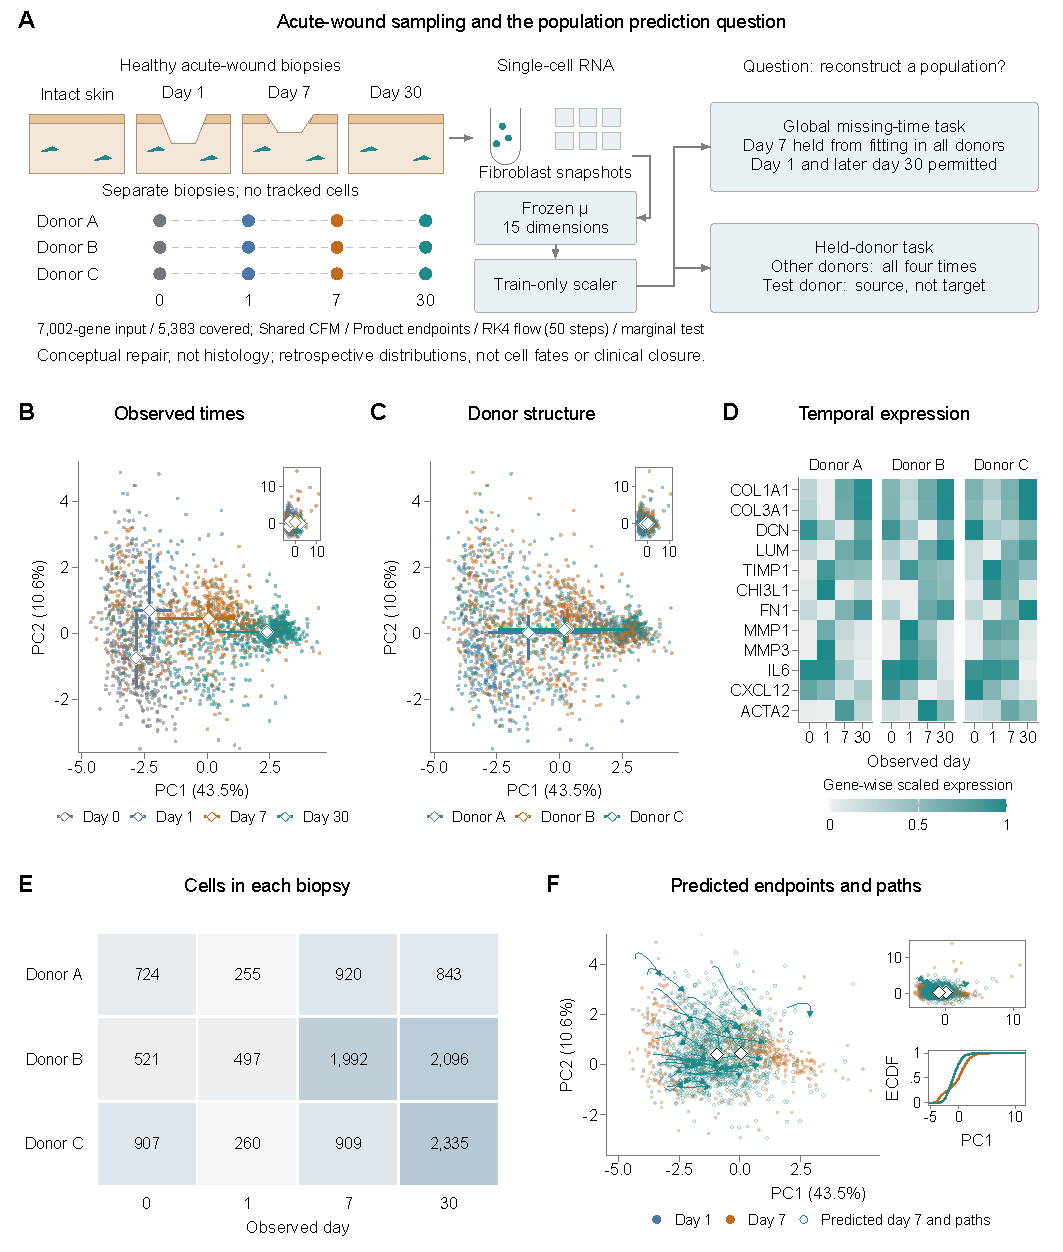
\includegraphics[width=\linewidth]{paper2_figure1_workflow.pdf}
\caption{What can acute-wound snapshots predict? (A) Conceptual repair and separate biopsies from three healthy donors at days 0, 1, 7 and 30; cells are not tracked. Global missing-time reconstruction excludes day 7 in every donor and permits later anchors. Held-donor transfer permits training-donor day-7 cells but excludes the test donor's target. Neither is clinical prognosis. A 7,002-gene input with 5,383 covered genes feeds frozen 15-dimensional μ, training-only scaling, product-endpoint CFM and 50-step RK4. Flow acts in scaled μ coordinates, not simplex weights. (B) Saved 2,000-cell display by time; day-7-excluded PCA explains 43.5\% and 10.6\% of training variance. (C) The same cells by donor. Diamonds/crosses denote medians/interquartile spans, not confidence intervals; focus windows retain full-range insets. (D) Twelve measured genes per biopsy, gene-wise scaled after pseudobulk normalization. (E) Recovered fibroblasts, not independent donors. (F) All 1,012 saved seed-0 endpoints, 36 numerical paths and observed day-1/day-7 display; insets show full range and PC1 cumulative distributions. Paths are not cell fates; errors use all 15 coordinates.}\label{fig:p2f1}\end{figure}

Matched raw-count profiles show the expression of matrix, inflammatory and contractile genes in each donor's four biopsies (Figure~\ref{fig:p2f1}D). Retained fibroblast counts differ across donor--time combinations (Figure~\ref{fig:p2f1}E), so neither point density nor the number of cells provides independent temporal replication. Projected paths connect observed day-1 starting coordinates to model-predicted coordinates at the prespecified day-7 time (Figure~\ref{fig:p2f1}F).

Display-subset medians and interquartile crosses summarize time and donor structure in the same projection (Figure~\ref{fig:p2f1}B--C). All saved predicted endpoints and a PC1 cumulative-distribution inset complement the paths (Figure~\ref{fig:p2f1}F); the observed comparison uses the display subset and is descriptive, not a replacement for full-coordinate scoring or a confidence region.

% Allow the next Results subsection to fill the text page while Figure 1
% remains on the immediately following float page (checked by build.py).
Joined fibroblast counts by donor and time are provided in Table~\ref{tab:p2biologicalcounts}.

\subsection{A held-out acute human time point can be reconstructed under the fixed protocol}

Global timepoint holdout removes day 7 from every donor, whereas donor transfer removes one donor and retains all four times in the others.

A fixed-seed refit assessed numerical resolution of the RK4 update in Supplementary equation~(S1) and sensitivity to evaluation sampling.

Using the empirical weighting rule in Equation~\eqref{eq:p2weighted} with all cells and the same fixed 50-step prediction, equal cell weights gave a 49.40\% improvement and equal donor mass gave 49.69\%.

The result is deliberately bounded.

Within-donor interpolation uses an observed later biopsy from the donor being reconstructed, which is permitted by the global timepoint-holdout task.

\FloatBarrier
Using the empirical version (Equation~\eqref{eq:p2edv}) of the energy discrepancy defined in Equation~\eqref{eq:p2ed}, the finalized held-out Wound7 analysis improved on the stay-still baseline by +49.9\% under Equation~\eqref{eq:p2improvement} (Figure~\ref{fig:p2f2}A\label{call:p2f2}). The held-out donor transfer analysis also passed in 3/3 folds, with a mean improvement of +75.9\% (Figure~\ref{fig:p2f2}B). In the geometry audit, the median same-donor temporal distance was 1.967 and the median same-time donor distance was 0.233, giving a time-to-donor ratio of 8.46 (descriptive 95\% resampling range 6.02--13.11; Figure~\ref{fig:p2f2}C).

\begin{figure}[htbp]\centering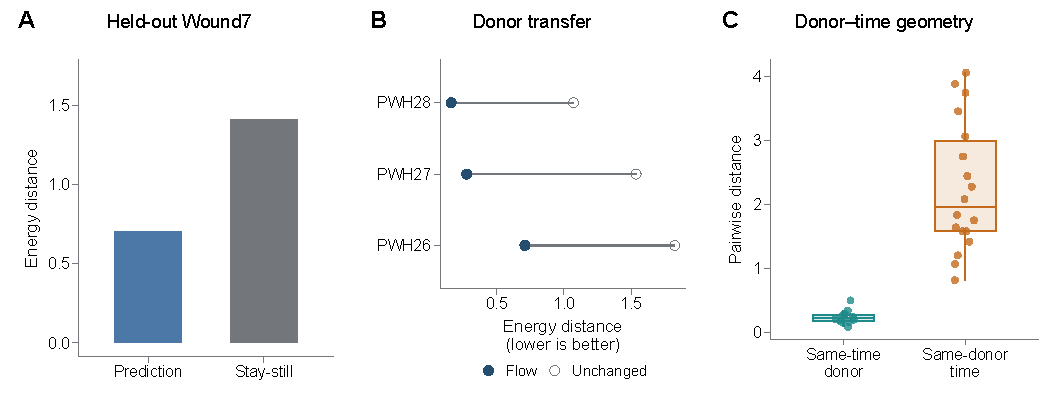
\includegraphics[width=\linewidth]{paper2_figure2_wound7_transfer.pdf}
\caption{Global Wound7 reconstruction, donor transfer and donor--time geometry. (A) Predicted and unchanged-source energy distances to pooled Wound7 after excluding that time globally; relative improvement is 49.9\%. (B) Connected filled and open points give predicted and unchanged-source errors for each genuinely excluded donor; the other two donors retain all four times. Mean relative improvement is 75.9\%, but absolute baseline and prediction errors differ by donor. These are point estimates, not confidence intervals. (C) Twelve same-time between-donor and 18 same-donor between-time distances, with interquartile boxes, medians and whiskers to observations within 1.5 interquartile ranges. The median temporal/donor ratio is 8.46; its 10,000-draw pair-distance resampling range is descriptive. All distances use training-standardized latent coordinates. Shared donors make pairs dependent, so these ranges have no established population coverage; three healthy donors do not validate DFU prediction.}\label{fig:p2f2}\end{figure}

Donor-specific reconstruction errors and descriptive geometry are detailed in Table~\ref{tab:p2folds} and Table~\ref{tab:p2geometrytable}.

\subsection{Simple interpolation is competitive when an entire time point is missing}

A retrospective extension tested whether improving over unchanged source requires a neural field.

For withheld day 7, unchanged source had mean donor error 1.4725. An independent-endpoint linear bridge gave 0.9284 (Figure~\ref{fig:p2f3}A\label{call:p2f3}). For withheld day 1, the unchanged-source error was 1.3460; shared flow, centroid translation and the independent bridge gave 1.0571, 0.9293 and 1.0959, corresponding to improvements of 21.5\%, 31.0\% and 18.6\% (Figure~\ref{fig:p2f3}B).

\begin{figure}[htbp]\centering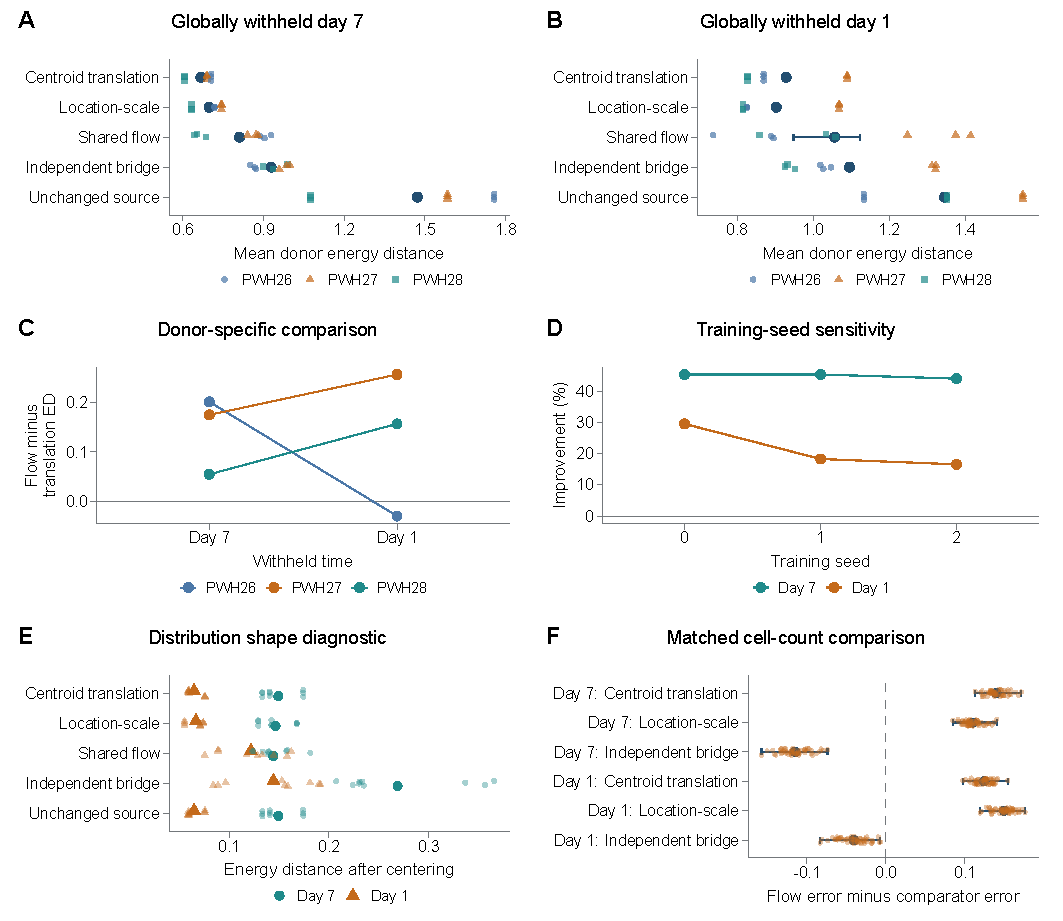
\includegraphics[width=\linewidth]{paper2_figure3_interpolation_controls.pdf}
\caption{Simple baselines for globally missing times. (A) Day 7 from day 1 with observed day 30 as anchor. (B) Day 1 from intact skin with observed day 7 as anchor. Large points are donor-macro means and bars span three seeds; smaller colored symbols retain individual donor/seed errors for all five predictors, including location--scale. Both tasks use rank-time fraction one half and are retrospective interpolation, not source-only prediction. (C) Donor-specific seed-averaged flow-minus-translation error. (D) Each flow seed's relative improvement. (E) Seed/donor-averaged centered energy distance with the individual donor/seed errors behind it; this is a shape diagnostic rather than additive error decomposition. (F) All 50 saved donor/seed-averaged paired draw contrasts, overlaid with means and ranges, using 200 source and target cells per donor. Positive differences favor the comparator. Seeds and draws are dependent computational evaluations of three donors; neither their ranges nor their point clouds are biological confidence intervals.}\label{fig:p2f3}\end{figure}

The centroid translation had lower seed-averaged error in all three donors for withheld day 7 and in two of three for withheld day 1 (Figure~\ref{fig:p2f3}C). Every fit improved over its unchanged source; Figure~\ref{fig:p2f3}D displays these seed-specific relative improvements.

The added comparison supports temporal information in the measured distributions, while providing no evidence that a neural field is necessary for the two interpolation tasks tested here.

The location--scale predictor in Equation~\eqref{eq:p2locationscale}, which interpolates endpoint standard deviations as well as means, gave errors of 0.6982 for day 7 and 0.9034 for day 1, also lower than the shared-flow errors in both tasks (Figure~\ref{fig:p2f3}A--B).

The distribution-shape diagnostics explain why a single aggregate error does not identify a uniform advantage. For day 1, flow had higher centered error (0.1220 versus 0.0647), while the independent bridge also had higher centered error (0.1445; Figure~\ref{fig:p2f3}E).

Matched 200-cell evaluation preserved the lower error of both deterministic endpoint controls in all 50 draws for each held time. Flow remained better than the independent bridge in every draw (Figure~\ref{fig:p2f3}F; Table~\ref{tab:p2matchedsampling}).

Pooled and donor-specific global missing-time comparisons are detailed in Table~\ref{tab:p2interpolation} and Table~\ref{tab:p2interpolationdonors}.

\subsection{Time parameterization changes the held-out result}

The historical single-seed, nearest-grid comparison gave linear days an improvement of −18.2\% relative to unchanged source (Table~\ref{tab:p2axes}). In the revised exact-time, three-seed paired-clock audit, the corresponding centroid translations gave 0.6667, 0.9775, 0.7476 and 0.6654, lower than the shared field under every clock on the donor-and-seed average (Table~\ref{tab:p2pairedclock}; Figure~\ref{fig:p2f4}A\label{call:p2f4}). Donor-specific flow-minus-centroid differences retain the heterogeneity behind this macro comparison (Figure~\ref{fig:p2f4}B).

\begin{figure}[htbp]\centering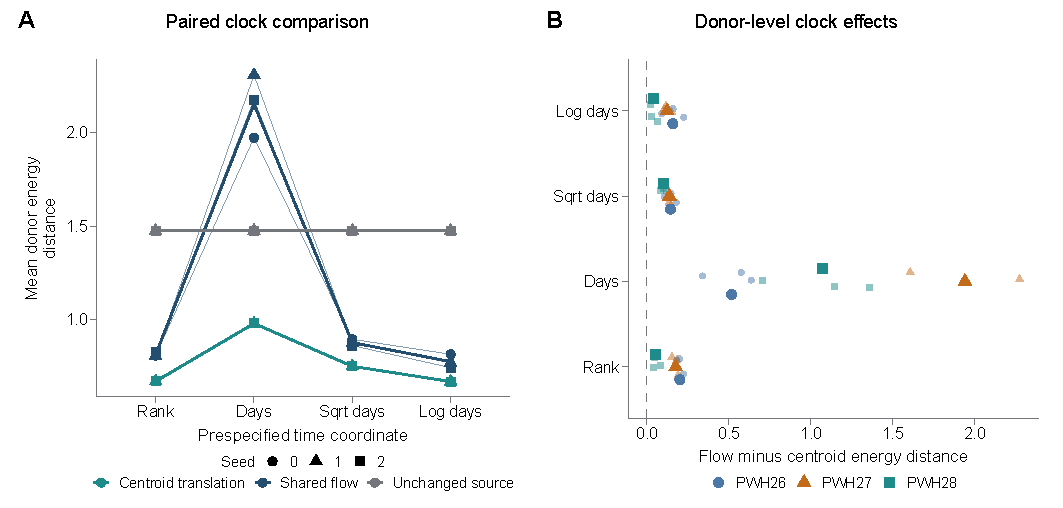
\includegraphics[width=\linewidth]{paper2_figure4_time_axes.pdf}
\caption{Paired time-coordinate sensitivity under global day-7 holdout in three healthy donors. Twelve fields cross four clocks with seeds 0, 1 and 2, each using 8,000 training steps and batch size 256. Initialization, endpoint draws and bridge random draws are paired across clocks within seed. Day 7 is excluded from fitting and scaling; 50 RK4 steps reach its exact transformed time, with identical evaluation rows and a 1,200-cell cap per donor. (A) Points are equal-donor means, shapes identify seeds, thin lines connect each seed and thick lines show seed means. Colors distinguish flow, centroid translation and unchanged source. Sqrt denotes square-root days; constant baselines overlap. (B) Large points show each donor's three-seed mean flow-minus-centroid error; small points retain the three seed-specific errors. Positive values favor the centroid and the dashed line marks no difference. Colors and shapes identify PWH26, PWH27 and PWH28 consistently across result figures. The centroid uses permitted day-1 and day-30 biopsies, so this remains retrospective interpolation. Clock connections are not biological trajectories; seed spread is not population uncertainty.}\label{fig:p2f4}\end{figure}

\subsection{The training-target distribution challenges the held-donor method ranking}

The historical held-donor benchmark gave shared flow matching a mean energy distance of 0.3947 (approximately 0.395) and gains above the split-half reference in 3/3 folds. The matched training-target marginal had mean error 0.1818, with a full range of 0.1479--0.2150 across 50 prediction-sampling draws (Figure~\ref{fig:p2f5}A\label{call:p2f5}).

The donor-specific results prevent a universal ranking: target-marginal mean errors were 0.1569, 0.1416 and 0.2469 for PWH26, PWH27 and PWH28, whereas shared-field errors were 0.7110, 0.2881 and 0.1850.

The context model in Equation~\eqref{eq:p2context} improved all 6/6 training-donor comparisons (Figure~\ref{fig:p2f5}B; Table~\ref{tab:p2insample}) while giving a higher held-out mean than the shared field.

\begin{figure}[htbp]\centering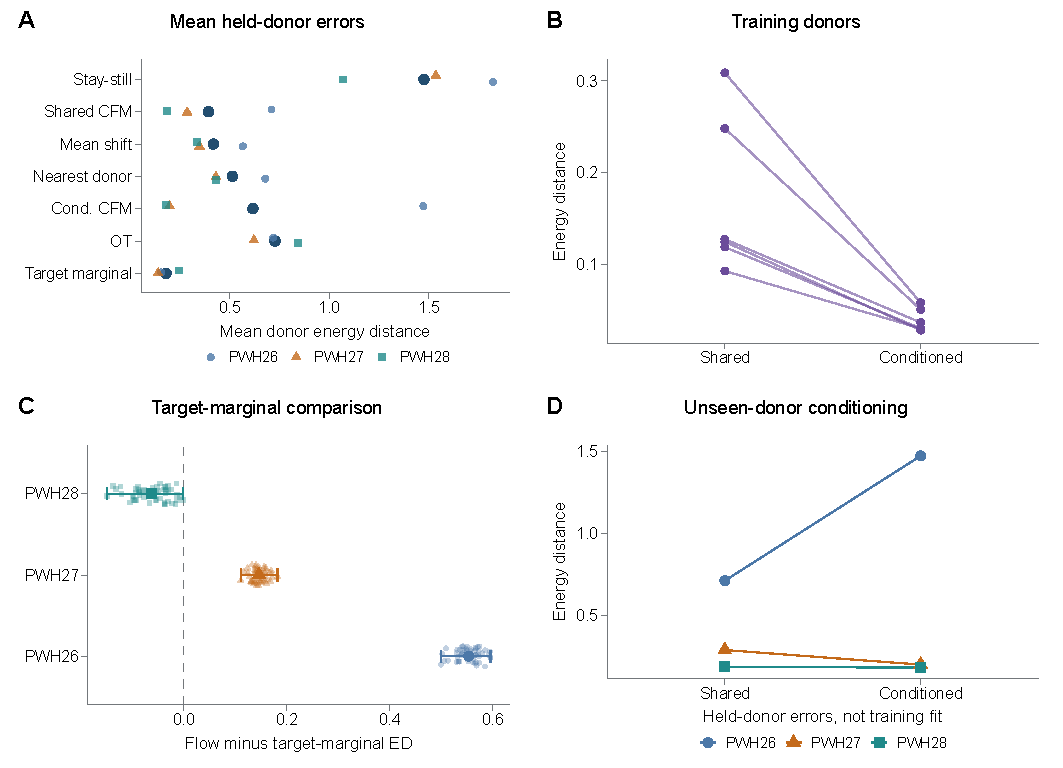
\includegraphics[width=\linewidth]{paper2_figure5_methods_benchmark.pdf}
\caption{Method means and donor-specific reversals in the historical held-donor benchmark. (A) Navy points are equally donor-weighted mean energy distances for unchanged source, five predictors and the added target marginal; smaller colored points retain all three donor errors for each method. CFM is conditional flow matching; OT is the separate entropic transport comparator. The marginal assigns equal mass to training-donor day-7 distributions without held-source expression; 50 matched-particle draws use the original target rows and scaling. (B) Six shared-versus-conditioned comparisons on training donors, all favoring conditioning; these are overlapping training observations, not transfer tests. (C) Each donor's fixed shared-field error minus the marginal's mean error, with the full 50-draw range and all 50 saved contrasts as smaller points. Positive values favor the marginal; PWH28 instead favors the field. These ranges describe prediction sampling, not donor-population confidence. (D) Connected shared and conditioned errors for the three genuinely held donors, separately exposing the gap between training fit and unseen-donor behavior. Historical neural/transport predictors used one training seed; the retrospective marginal audit does not establish a stable method ranking.}\label{fig:p2f5}\end{figure}

The donor-specific marginal comparison shows its full prediction-sampling range and the reversal in PWH28 (Figure~\ref{fig:p2f5}C). Comparing the shared and conditioned fields in genuinely held donors (Figure~\ref{fig:p2f5}D), rather than only training donors, prevents improved training fit from being read as generalization evidence.

The original neural and transport method comparison used one training seed and successive endpoint random draws.

Pooled and donor-specific method comparisons are detailed in Table~\ref{tab:p2methods} and Table~\ref{tab:p2methodsbydonor}.

\subsection{Donor-count comparisons require a common evaluation scale}

The initial count curve changed its standardization when the training subset changed, so subtracting its absolute errors mixed information gain with a change of distance geometry.

A rerun with one fixed training-derived evaluation geometry compared one and two training donors. The same common geometry showed lower error for mean displacement (0.5095 to 0.4186), the full equal-donor target marginal (0.2222 to 0.1676), and its matched-particle version (0.2332 to 0.1818).

Figure~\ref{fig:p2f6}A\label{call:p2f6} shows all three seeds and the seed-0 line (0.5315 to 0.3854). Seed-specific reductions were 0.1462, 0.1558 and 0.1430 (Figure~\ref{fig:p2f6}B).

\begin{figure}[htbp]\centering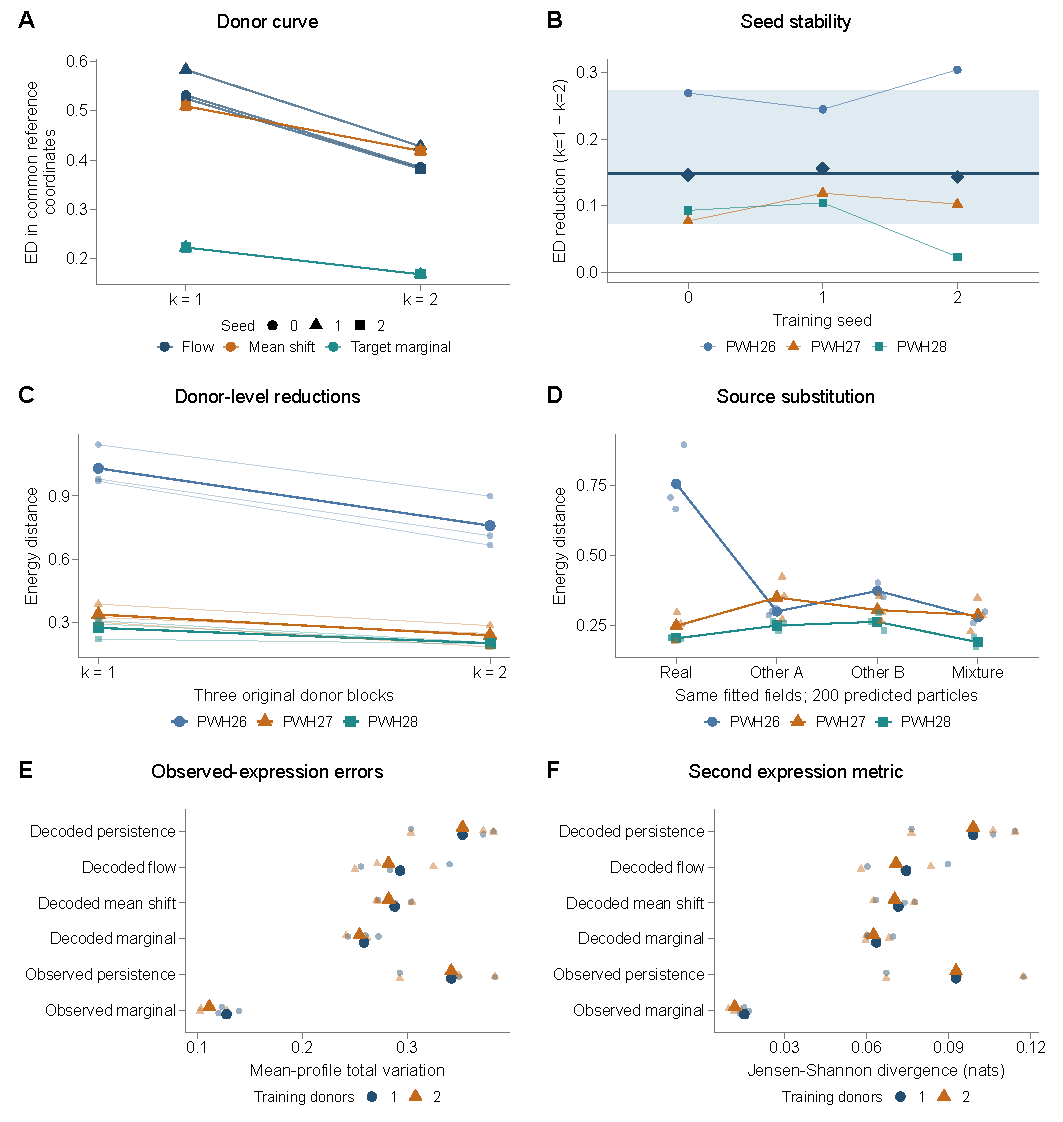
\includegraphics[width=\linewidth]{paper2_figure6_donor_curve_stability.pdf}
\caption{Donor count, source substitution and observed-expression restrictions. (A) Three-seed shared-flow curves alongside saved mean-displacement and exact target-marginal curves, in the same reference geometry and hierarchical donor weighting. (B) Macro seed reductions (navy diamonds; navy line, their mean), all nine donor/seed reductions and the saved descriptive three-block 95\% range; shading is not a seed-level interval. (C) Donor means with finer seed-resolved curves. (D) Real source, each alternative donor and their mixture under the saved 200-particle, 50-draw protocol; large points are donor means and smaller points are the three seed means. Other A/B are sorted alternatives within each fold. (E) Total variation against observed mean expression on 5,383 common genes. (F) Jensen--Shannon divergence for the same predictions. E/F distinguish decoded and directly observed predictors; large symbols are equal-donor macros and faint symbols are three donor means after seed/subset averaging, for each training size. Source mixing is not a donor-count experiment, and mean-expression errors are not full cellular-distribution validation. All panels reuse three donors; seeds, draws and overlapping folds add no biological replication.}\label{fig:p2f6}\end{figure}

The donor-resolved curves retain the unequal reductions within the same three blocks (Figure~\ref{fig:p2f6}C). The separate 200-particle source audit distinguishes each individual alternative from their mixture (Figure~\ref{fig:p2f6}D); it is a sensitivity analysis of fixed fields, not another donor-count experiment.

The saved two-donor fields also allow the starting distribution to be changed without changing training, target cells or scoring scale.

The exact target-marginal reduction was 0.054601 across donors and matched one quarter of the training-target mutual discrepancy, with maximum numerical residual below $2.45\times10^{-15}$ (Table~\ref{tab:p2mixtureidentity}).

Within a fixed donor and training subset, the mean training SD was 0.0701, or 3.07 times the mean split-half reference of 0.0228; the largest seed range was 0.3377 (Table~\ref{tab:p2seedconfigs}).

Common-coordinate donor-count results and their seed-averaged summaries are detailed in Table~\ref{tab:p2curve} and Table~\ref{tab:p2seedcurve}.

\subsection{Observable expression errors do not establish a flow advantage over target marginals}

Raw-expression alignment and frozen re-encoding passed for all 12,259 cells, with maximum encoder-mean discrepancy $1.91\times10^{-6}$. Against observed target mean expression, the directly observed training-target marginal gave total-variation errors of 0.1279 and 0.1115 with one and two training donors, compared with 0.2590 and 0.2546 for its decoded form; these controls do not use the excluded donor's source expression (Figure~\ref{fig:p2f6}E; Table~\ref{tab:p2observable}). At two training donors, decoded flow had total variation close to decoded mean displacement, while its Jensen--Shannon divergence was higher (Figure~\ref{fig:p2f6}F), so these metrics do not establish a consistent neural advantage.

The decoder reconstruction reference for observed target cells is provided in Table~\ref{tab:p2decoderreference}.

\subsection{Finite-budget PCA diagnostics preserve the baseline concern}

The separate train-PCA diagnostic completed all 48 flow fits and 12 baseline jobs across the same three donors.

Longer budgets generally reduced unconditioned flow errors, but not every conditioned donor comparison improved.

\subsection{Three mouse arms expose model-arm heterogeneity}

The all-arm audit gave different results under the same protocol, using the endpoint-distance diagnostic in Equation~\eqref{eq:p2geometry}. In aggregate, 2/3 arms beat stay-still, 2/3 met the noise criterion and 2/3 satisfied the ordering check (Figure~\ref{fig:p2f7}A\label{call:p2f7}).

The paired baseline and predicted distances show the absolute error scale within each mouse arm (Figure~\ref{fig:p2f7}B); relative improvement alone would hide these differences.

The complete arm--time cell counts expose unequal recovery (Figure~\ref{fig:p2f7}C), while separate baseline, noise and endpoint-ordering outcomes retain every failed diagnostic (Figure~\ref{fig:p2f7}D).

\begin{figure}[htbp]\centering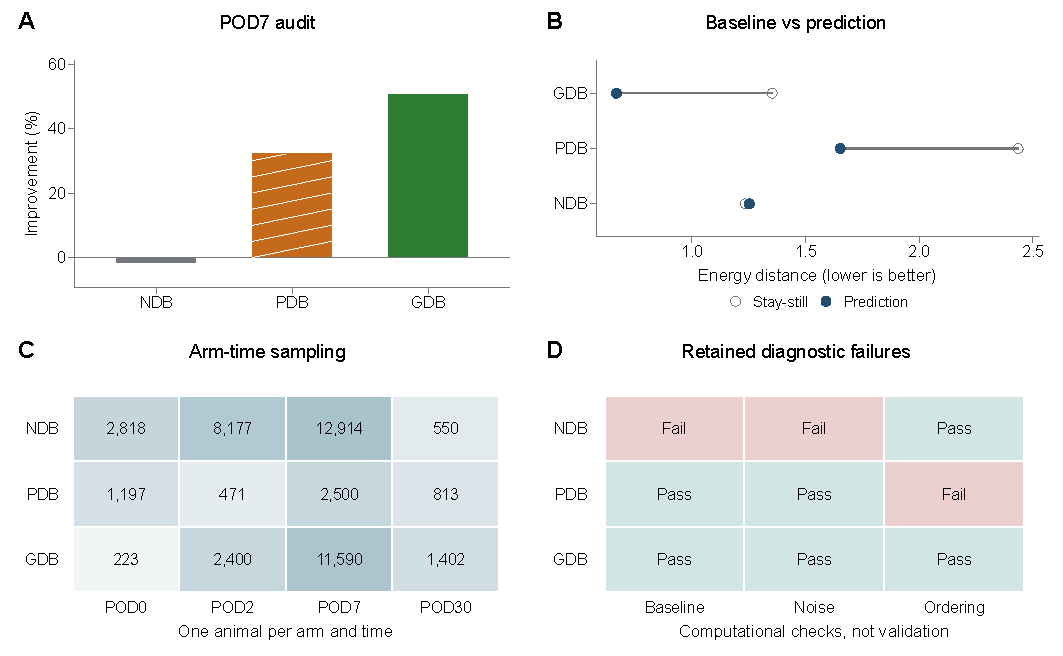
\includegraphics[width=\linewidth]{paper2_figure7_mouse_arms.pdf}
\caption{Mouse POD7 computational audit for NDB, PDB and GDB source arms. POD7 is excluded from fitting and scaling; fields trained at POD0, POD2 and POD30 predict from POD2. (A) Relative improvements −1.5\%, +32.1\% and +50.6\%; PDB hatching marks the failed endpoint-ordering check. (B) Connected unchanged-source and prediction errors on the absolute scale. (C) All 12 saved arm-time cell counts; color follows log-count and printed values are exact counts. Each entry has one animal, not multiple biological replicates. (D) Separate baseline, split-half noise and endpoint-ordering check outcomes, preserving every failure. Neither pass labels nor endpoint ordering establish biological trajectories. All arms cover 4,182/7,002 panel genes; no biological confidence intervals are available, and cells are not independent animals or clinical validation.}\label{fig:p2f7}\end{figure}

Mouse fibroblast counts and model-arm errors are detailed in Table~\ref{tab:p2mousecounts} and Table~\ref{tab:p2mouse}.

\subsection{Symmetric repeated evaluation preserves donor and information-set differences}

All 107 jobs passed original-backend replay with zero maximum prediction discrepancy.

Three population-transport draws emitted Sinkhorn iteration warnings.

The source-bound repeated experiment completed all 107 planned fitted jobs, retaining all permitted comparators and three neural seeds under a common architecture and 8,000-step optimizer budget.

\Needspace{5\baselineskip}
These results retain the near-parity and contrary comparisons rather than asserting universal neural inferiority (Figure~\ref{fig:p2f8}A\label{call:p2f8}; Table~\ref{tab:p2qualitymissing}).

Held-donor ratios instead use the observed training-target marginal, with day-1-to-day-7 results displayed separately and all adjacent intervals retained numerically (Figure~\ref{fig:p2f8}B; Table~\ref{tab:p2qualitydonor}).

\begin{figure}[htbp]\centering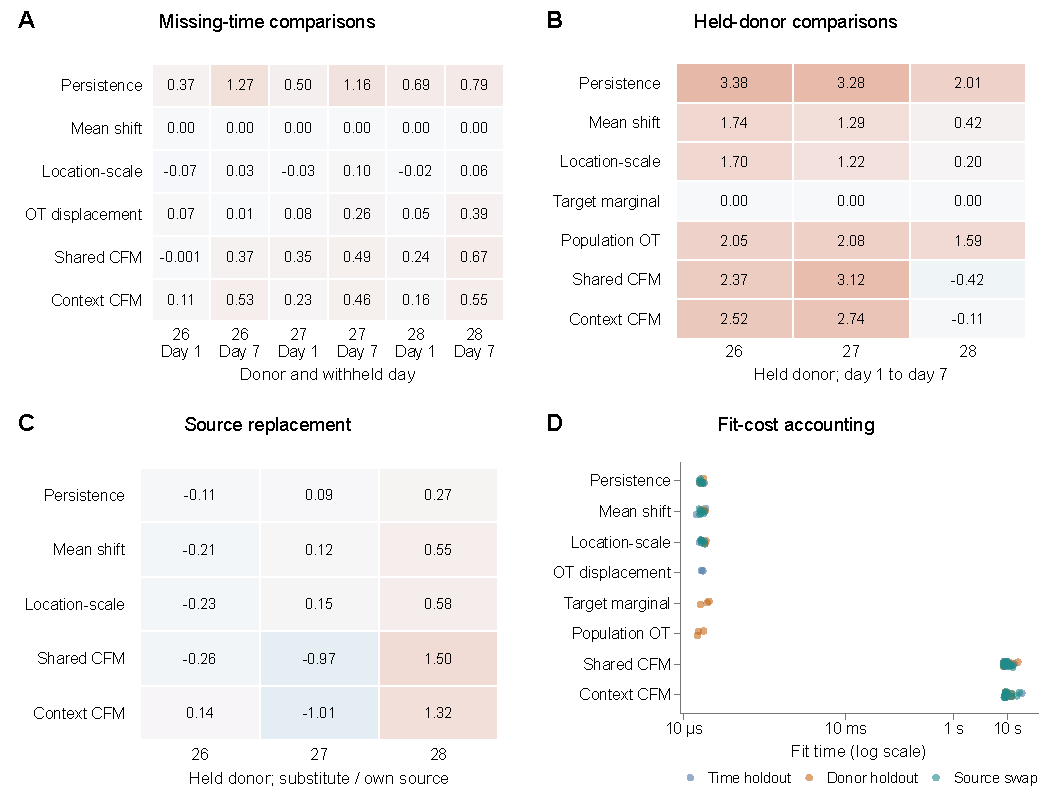
\includegraphics[width=\linewidth]{paper2_figure8_paired_comparison.pdf}
\caption{Source-bound repeated comparisons in the frozen representation. (A) Each cell is the mean paired log2 energy-error ratio to mean translation within a donor and withheld day, averaging 50 matched draws within a fit and then three neural training seeds. (B) Day-1-to-day-7 donor-transfer ratios use the permitted equal-training-donor target marginal instead. Negative values favor the row method; zero denotes its comparator. Neither display pools raw distances from differently standardized donor folds. (C) Source replacement divides each substituted-source error by the own-source error from the same field and target draw, then averages draws, seeds and the two substitute choices within donor. These separate fits exclude both the held donor and the substitute from fitting; positive values indicate lower error from the own source. (D) Every one of the 107 fitted-job timings is counted once, not once per evaluation draw; colors distinguish missing-time, held-donor and source-replacement tasks. Fit time excludes representation setup, prediction, scoring and input/output and is not an equal-compute comparison. Original-CUDA-backend replay and the failed CPU portability check are distinguished. All panels reuse three healthy acute-wound donors, without inferential method ranking or clinical validation.}\label{fig:p2f8}\end{figure}

Source-replacement ratios compare the substituted and own source from the same field and target draw, retaining every donor, seed and substitute choice (Figure~\ref{fig:p2f8}C).

Fit costs count each fitted job once (Figure~\ref{fig:p2f8}D).

Two warning draws were PWH27 day-0-to-day-1 draws with both returned marginals inside the fixed audit tolerance; the PWH26 day-7-to-day-30 draw had column L1 residual $1.061\times10^{-6}$, above the $10^{-6}$ bound, while its row residual was below $1.12\times10^{-16}$.

\subsection{A cross-sectional mouse series admits one population for withheld-day reconstruction}

The hashtag audit separates what GSE186527 can and cannot support (Table~\ref{tab:p2extlibraries}).

For that population, POD14 reconstruction from POD7 with a POD30 anchor gave energy 0.441 for stay-still and 0.343 for the declared location--scale comparator (Table~\ref{tab:p2extresults}).

Scoring each prediction against the four held mice separately shows the scale of the nesting (Table~\ref{tab:p2extscale}).

A second execution of the same nominal protocol and seeds saved reloadable fitted states for all 19 fits (Table~\ref{tab:p2extrepeat}).

Primary and sensitivity hashtag counts are detailed in Table~\ref{tab:p2extgroups}.

\subsection{Coupling and coordinates alter errors without establishing a consistent neural advantage}
The additional human follow-up retained every declared fit. All 354 original fields and nine selected outer refits reproduced their full-source predictions exactly on CUDA; all 31 cached coordinate matrices also reproduced exactly from the input. A separate recomputation matched 2,700 deterministic-control evaluation rows to within $4.5\times10^{-16}$. These checks support the saved computations, with the retrospective training-provenance and alpha-grid limits stated in Methods. The earlier CPU-portability failure remains unresolved.

For missing day 7, OT-coupled log2 energy ratios to translation were $-0.026$, 0.321 and 0.351 in PWH26, PWH27 and PWH28; entropic-bridge ratios were 0.016, 0.284 and 0.192 (Figure~\ref{fig:p2f9}A\label{call:p2f9}; Table~\ref{tab:p2followcoupling}).

Across all five coordinate systems, the donor-mean day-7 ratio favored translation for both independent and OT fields (Figure~\ref{fig:p2f9}B; Table~\ref{tab:p2followrepresentation}).

\begin{figure}[htbp]\centering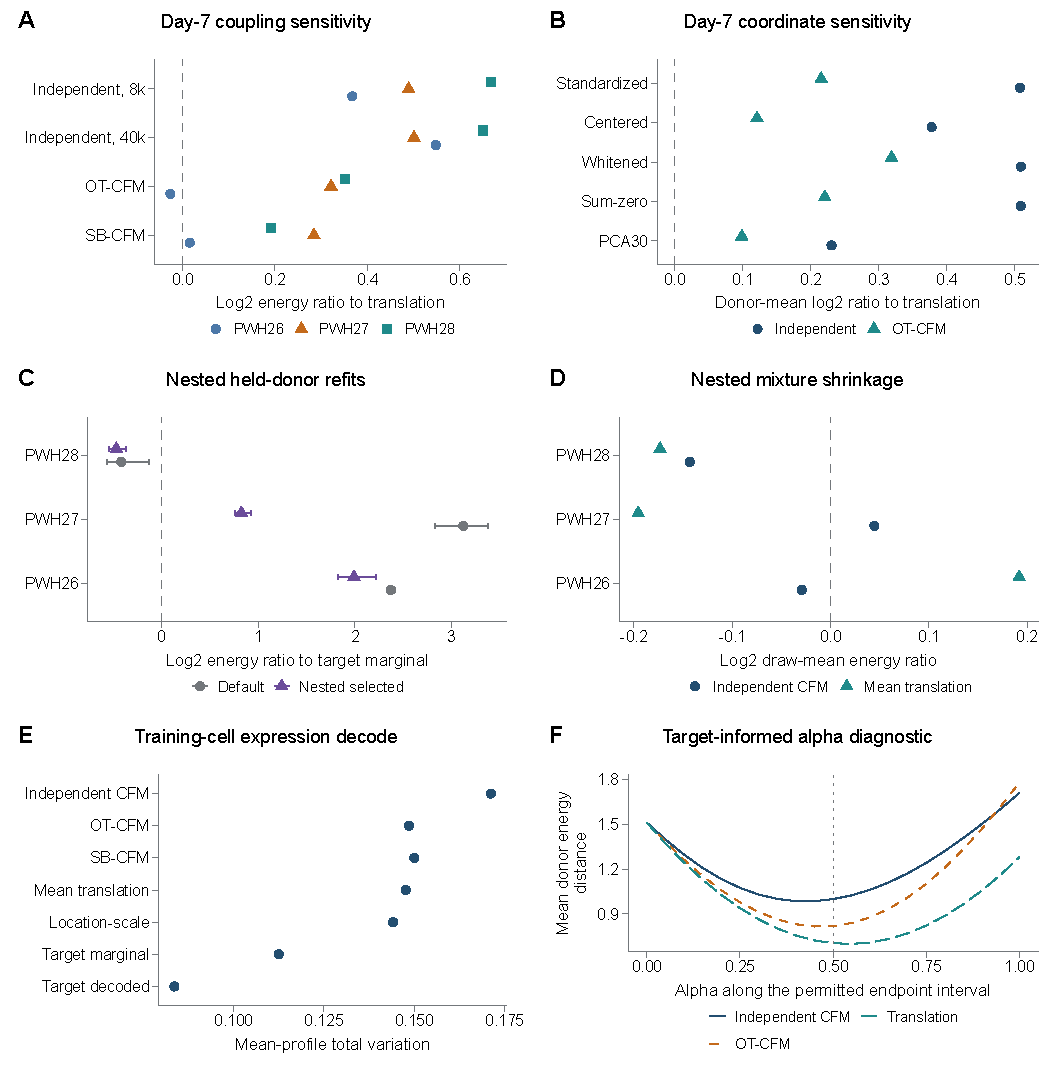
\includegraphics[width=\linewidth]{paper2_figure9_followup.pdf}
\caption{Completed computational follow-up. (A) Missing-day-7 log2 energy ratios to translation in each donor, across coupling families and two independent-field budgets. (B) Donor-mean day-7 ratios in five training-fitted coordinate systems. (C) Default and nested selected day-1-to-day-7 fields relative to the training target marginal; whiskers span three seed means. (D) Nested mixtures of transported source and target marginal, using log2 ratios of draw-averaged energies, a different estimand from A--C. (E) Held-donor mean-expression errors after mapping predictions to 15 nearest permitted training cells; decoding observed target cells supplies a reference. (F) Target-informed alpha scans of fixed rank-trained predictors, with rank alpha 0.5 dotted. Alpha optima are retrospective diagnostics. All panels reuse three human donors; draws and seeds add no biological replication.}\label{fig:p2f9}\end{figure}

Nested selection reduced held-donor day-1-to-day-7 errors compared with the default field, while leaving the comparison with the target marginal donor-specific (Figure~\ref{fig:p2f9}C; Table~\ref{tab:p2follownested}).

The nested mixture in Equation~\eqref{eq:p2shrinkage} also retained contrary results (Figure~\ref{fig:p2f9}D; Table~\ref{tab:p2followshrinkage}).

Training-cell decoding gave held-donor mean-expression total variation of 0.171 for independent flow, 0.149 for OT flow, 0.144 for location--scale and 0.113 for the target marginal (Figure~\ref{fig:p2f9}E; Table~\ref{tab:p2followdecode}).

The target-informed alpha scan found a day-7 donor-mean minimum at alpha 0.55 for translation and 0.45 for OT flow (Figure~\ref{fig:p2f9}F; Table~\ref{tab:p2followalpha}).

\section{Discussion}

Coupling variants and nested model selection qualify the interpretation of the default neural field. The completed outer refits reduced its errors, but selected fields still lost to the training target marginal in two of three held donors and improved in the third.

The symmetric repeated comparison confirms the baseline concern without making it universal. Missing-day-7 reconstruction favored mean translation in every neural donor--method mean, while held-donor day-7 reconstruction favored neural fields over the target marginal for PWH28 but not PWH26 or PWH27.

The global missing-time comparison changes the interpretation of model complexity. A within-donor mean translation had lower average error than the shared field for both withheld times, even though the field improved over an unchanged source.

The donor-holdout task exposes a further baseline requirement. Because the target time is observed in training donors, their empirical target distributions can supply a prediction without using the excluded donor's starting expression.

The observed-cell maps and biopsy expression profiles make the population being transported more concrete, but they do not establish a lineage or wound mechanism. A two-dimensional projection omits variation even when fitted solely to training cells \citep{huang2022visualization}.

The learned field is a model of distributions under a specified sampling construction. Independent endpoint cells from the same donor define linear paths and regression targets; those pairings are not observed cell lineages or an estimated minimum-cost coupling.

Additional biological measurements would constrain a different part of the problem. Lineage tracing relates ancestry to later cell states, whereas RNA velocity derives directional information from transcript processing under a kinetic model \citep{weinreb2020,lamanno2018,bergen2020}.

Normalization to a probability distribution introduces another biological limit. Wound repair involves proliferation, loss, recruitment and matrix remodeling, with experimental evidence for coordinated fibroblast and macrophage responses \citep{rognoni2018,shook2018}.

The time-axis comparison identifies a consequential modeling choice. The revised three-seed audit pairs the random streams and integrates to the exact target, addressing defects in the original single-seed comparison.

Donor conditioning improved the fit to known donor contexts without improving the overall held-out mean relative to the shared field. Additional context can increase fitting capacity while also creating an extrapolation problem for an unfamiliar donor.

The distance used for evaluation also determines the interpretation of improvement. Energy distance compares distributions through pairwise geometry and has a formal relationship to kernel discrepancies \citep{szekely2013,sejdinovic2013}.

The fitted and evaluated donor measures also differ. Cycling through donor--segment pairs approximately balances training contributions, whereas pooled evaluation weights cells according to yield.

Numerical integration and evaluation sampling were stable over the tested settings for one fixed field. Increasing Runge--Kutta resolution changed the coordinates negligibly, and repeated subsampling preserved improvement.

The finite-budget train-PCA diagnostic extends the baseline concern across multiple coupling variants and both budgets in all three donors. It remains a separate experiment: preprocessing, architecture, intervals and optimization settings differ from the primary frozen-coordinate analysis.

An external mouse series was admitted narrowly. Three of four arm and gate tasks failed the frozen 50-cell floor at the last time point, and the unwounded and POD2 libraries could not be assigned because no hashtag counts were released.

The mouse arms had different errors, one animal per time and incomplete panel coverage; time, animal and representation effects remain entangled. Neither acute human nor mouse wounds supply independently observed diabetic-foot-ulcer courses \citep{armstrong2017}.

\section*{Additional Information}
Funding. No funding was received for this study.

Competing interests. The author declares no competing interests.

\section*{Author contributions}
Zeyu Fu conceived the study, developed the methodology and software, curated the public data, performed and verified the analyses, prepared the visualizations, and wrote and revised the manuscript.



Consent for publication. The article contains no identifiable individual information or participant images. The tissue drawings are conceptual illustrations.

\section*{Data Availability}
Public processed counts and author annotations are available from NCBI Gene Expression Omnibus as GSE241132 (acute human wounds), GSE165816 (the frozen expression representation) and GSE326622 and GSE186527 (mouse wounds). GSE165816 clinical labels are not used to fit temporal fields. Numerical tables accompany this article; the study repository's Releases page provides the current versioned reproduction package, including derived results, frozen models, editable figures and acquisition instructions. Its reproduction scope is stated below. No request to the author is required. Raw GSE241132 human sequencing reads remain under controlled access through the European Genome--phenome Archive.

\section*{Code availability}
Current analysis software, numerical evidence, saved evaluation inputs and reproduction instructions are available at \url{https://github.com/PeterPonyu/wound-population-dynamics} and archived at software DOI \url{https://doi.org/10.5281/zenodo.23308074}. The archive manifest identifies the included checkpoints and analysis records. Source-study inputs retain their original terms.

The current archive includes the revised analyses and documented saved-state evidence. Earlier immutable archives identify earlier software releases. Document reconstruction, verification of saved numerical evidence and fresh model fitting are separate tasks; full fitting requires the specified upstream inputs and computing environment. No additional biological replication is claimed by packaging.

Acknowledgements. The author thanks the original investigators and participants for making the source datasets available.
\FloatBarrier
\bibliographystyle{unsrtnat}
\bibliography{references_paper2}
\end{document}